\chapter{Including dispersal}
\label{ch5:dispersal-model}

In the previous Chapter, we employed a simple lattice model (SLM) based on percolation. The percolation setting provided a tractable starting place. Nevertheless, several limitations underpinned the model. Chiefly, percolation models rest on local, nearest-neighbour (NN) contacts and cannot describe epidemics at lower, more realistic tree densities ($\rho \sim 0.10$). Subsequently, this Chapter will generalise the SLM and incorporate non-local NN interactions by introducing a generic Gaussian dispersal kernel, allowing epidemics at far lower tree densities.

The thin-tailed Gaussian kernel introduced here represents an intermediate step between the NN interactions in the SLM and the fat-tailed inverse power-law dispersal present in Chapter \ref{ch:6-adb}. The ease of integrating a Gaussian kernel also proved helpful when deriving an analytic expression of $R_0$, as discussed more below. Other choices of simple one parameter dispersal kernels are possible, including the slightly longer range negative exponential\textemdash discussed at length in \cite{nathan2012dispersal}. Regardless, any developing epidemic that follows a similar ranged kernel will ultimately approximate similar spreading patterns \cite{bullock2017synthesis}.

Firstly, we will combine dispersal-based interactions within a simplistic SIR framework to construct a non-local model (NLM) of tree disease. The model behaviour is then examined under various dispersal length scales and fitted against the standard SIR to contrast disparities between spatial and non-spatial models.
After establishing the non-local dispersal model, a spatially explicit (analytic) expression for the basic reproduction number will be derived for the model, denoted by $R_0$. 

Next, we compare analytical predictions of $R_0$  against the total tree mortality, equivalent to the final-sized epidemic. Lastly, the expression of $R_0$ is scrutinised against the `actual' number of secondary infections, computed by contact-traced individual tree-to-tree infections. Notably, the analytic and contact-traced methods of calculating $R_0$ define a threshold at $R_0=1$. As before, the analysis is kept generic, with arbitrary units of time and distance, before incorporating more biological realism in the next Chapter.

\section{A small-scale non-local SIR model}
\label{section:sgm-expo}

As before, we begin with a model fixed inside a square lattice of size $\mathcal{L}$ and host units refer to individual trees. Host distributions are initialised by a Bernoulli trial with probability $\rho$ according to a binomial distribution. Thus, the probability of host occupation ($\rho$) can be seen as a tree-density parameter and interactions between hosts are modelled over a flat and randomly distributed population.
The state of a tree can be in one of three conditions: susceptible, infected, or removed (SIR).
We assume all trees are equally susceptible, and trees that become infected transition through the states $S\rightarrow I\rightarrow R$ without the possibility of recovery.

From first principles, the probability of infection at a distance $r$ can be described by an unnormalised Gaussian function $g(r; \ell)$, where $\ell$ is a distance that sets the scale of dispersal. 
If two trees\textemdash one susceptible ($S_x$) and one infected ($I_{x^\prime}$)\textemdash are separated by a distance $r=|x - x^\prime|$, then a transition probability between the states $S_x \rightarrow I_x$ can be defined by the $g(r; \ell)$ multiplied by infectivity $\beta$:
\begin{equation}
\label{eq:pr-dispersal-transition}
    Pr(S_{x} \rightarrow I_{x} ;\ I_{x^{\prime}} ) = \beta \exp\Big[\frac{-r^2}{2\ell^2}\Big]
\end{equation}
where $\beta$ is interpreted as a probability, i.e. $\beta \in [0, 1]$. 
Equation \ref{eq:pr-dispersal-transition} generalises the SLM to include non-local interactions, hence referred to as the non-local model (NLM).
Each probability of transition is assessed against a sample drawn from a continuous uniform distribution $U(0, 1)$ following a Poisson construction \cite{cook2008constructing}. 
Probabilities are then calculated for each times step while host $S_x$ 
remains susceptible, and repeated for each susceptible tree in the domain (i.e. $\forall S_x \in [\mathcal{L}, \mathcal{L}]$).
See Appendix \ref{A:combiniing-probabilities} for more information on the computational implementation. A table of parameters for the NLM is shown below in Table \ref{tab:SIR-model}.

The same uniform lifetime dynamic (used previously in the SLM) controls the period hosts remain infectious.
That is, a host transitioning into the $I$ compartment will remain infectious for $T$ time steps before uniformly transitioning into the $R$ compartment.
In section \ref{ch3:two-param-model}, the infection period was shown to alter the wave-front thickness and the threshold value of infectivity $\beta$ required for an epidemic. 
However, an arbitrary number of $T=100$ infectious time steps remains fixed throughout this Chapter.
Uniform transitions into the $R$ compartment help to keep the model simple but present an assumption that goes against the grain of more common exponential lifetime dynamics\textemdash discussed more below in section \ref{sec:SIR-fitting}.

\begin{table}
\centering
\begin{tabular}{l l l}
\hline
\textbf{Model parameter} & \textbf{Description} & \textbf{Typical value(s)}\\
\hline
$\rho$  & Tree density & $0.00 - 0.10$ \\ 
$\beta$ & Infectivity probability & $0 - 10^{-3}$ \\
$\beta^*$ & Auxiliary infectivity & $0 - 10$ \\
$\ell$ & Gaussian dispersal parameter & $ 0 - 100$ \\
$t$ & Simulation time step & $1\ \mathrm{Au}$\\
$T$ & Infectious life time & $100$  \\
$\alpha$ & Lattice constant & $1\ \mathrm{Au}$ \\
$\mathcal{L}$ & Square lattice dimension & $200$ - $2000$ \\
$R_0$ & Basic reproduction number & $0-20$ \\
$R_0^{(i)}$ & Generational reproduction number & $0-20$ \\
\hline
\end{tabular}
\caption{Parameters used in the generic NLM, time and distance are given in arbitrary units and host densities are informed from by \cite{hill.data}.}
\label{tab:SIR-model}
\end{table}

The work presented in this Chapter is purposefully kept generic, with no specific pathogen in mind.
Therefore, each Monte Carlo step through the simulation has arbitrary units of time and distance.
Nevertheless, the units of time and distance can be envisioned to be on the order of days and meters to reflect the approximate spatio-temporal scale of general tree disease.
As demonstrated later in Chapter \ref{ch:6-adb}, spatial scale within the model can be calibrated by choosing a suitable lattice constant, denoted by $\alpha$, that reflects the size of host units.

\newpage 

\section{Model behaviour}

Spatio-temporal epidemic progression within the NLM is depicted in Figure \ref{fig:sgm-evol}.
Figures \ref{fig:sgm-evol}(a-b) depict an epidemic spreading through the domain at two time steps;
simulation parameters are given by $\rho=0.01,\ \ell = 25,\ \beta = 1.0 \times 10^{-3}$ on a domain of size $500 \times 500$.
All panels in Figure \ref{fig:sgm-evol} begin from a small number of infected hosts at the domain centre at $t=0$.
A tree density of $\rho = 0.01$ approximately mirrors the median canopy coverage of a large deciduous tree distributed throughout the GB, according to the predicted oak abundance data given by \cite{hill.data}\textemdash presented previously in Figure \ref{fig:uk-oak-l.hill}.
Unsurprisingly, extending the neighbourhood of interaction to non-nearest neighbours permits an epidemic for much lower tree densities in comparison to the SLM percolation threshold studied in Chapter \ref{chapter:SLM}.

Figures \ref{fig:sgm-evol}(a-b) suggest an approximate wave-front-like behaviour, as infections spread out radially from the epicentre.
The corresponding ensemble-averages of Figures \ref{fig:sgm-evol}(a-b) are shown below in Figures \ref{fig:sgm-evol}(c-d), and confirms a travelling wave-like spread.
For 200 repeated simulations, the spatial locations of infected trees were recorded and plotted as a two-dimensional frequency distribution.
The upper and lower marginal plots of Figures \ref{fig:sgm-evol}(c-d) show the one dimensional horizontal and vertical frequency distributions, respectively.
Disease progression in Figure \ref{fig:sgm-evol}(d) reflects the radial propagation of a travelling wave and a disease gradient of approximately $\approx 3\ell$.
Thus, choosing a small value of $\ell=25$ in comparison to the domain effectively recovers the essential wave-like behaviour exhibited by the SLM.

The thin-tailed Gaussian kernel does not permit the pathogen to jump large discontinuous distances, particularly for a small value of $\ell=25$, as shown in Figure \ref{fig:sgm-evol}. Therefore, we can present an analogy to percolation provided that the ratio $\frac{\ell}{\mathcal{L}}$ is small, allowing us to calculate a wavefront similarly to the method described previously in Chapter 3. Accordingly, Figure \ref{fig:sgm-evol}(e) reveals the largest distance an infected host will likely reach over 500 steps. Boundary conditions in Figure \ref{fig:sgm-evol}(e) terminate simulations upon three conditions: 
(A) The simulation time step exceeds 500 steps 
(B) No infected trees remain in the domain 
(C) An infected tree $I_{x}$ falls within a distance $\mathcal{L} - 3\sigma_{ga} \leq I_{x} \leq \mathcal{L}$ away from the epicentre.
    
\begin{figure}
    \centering
    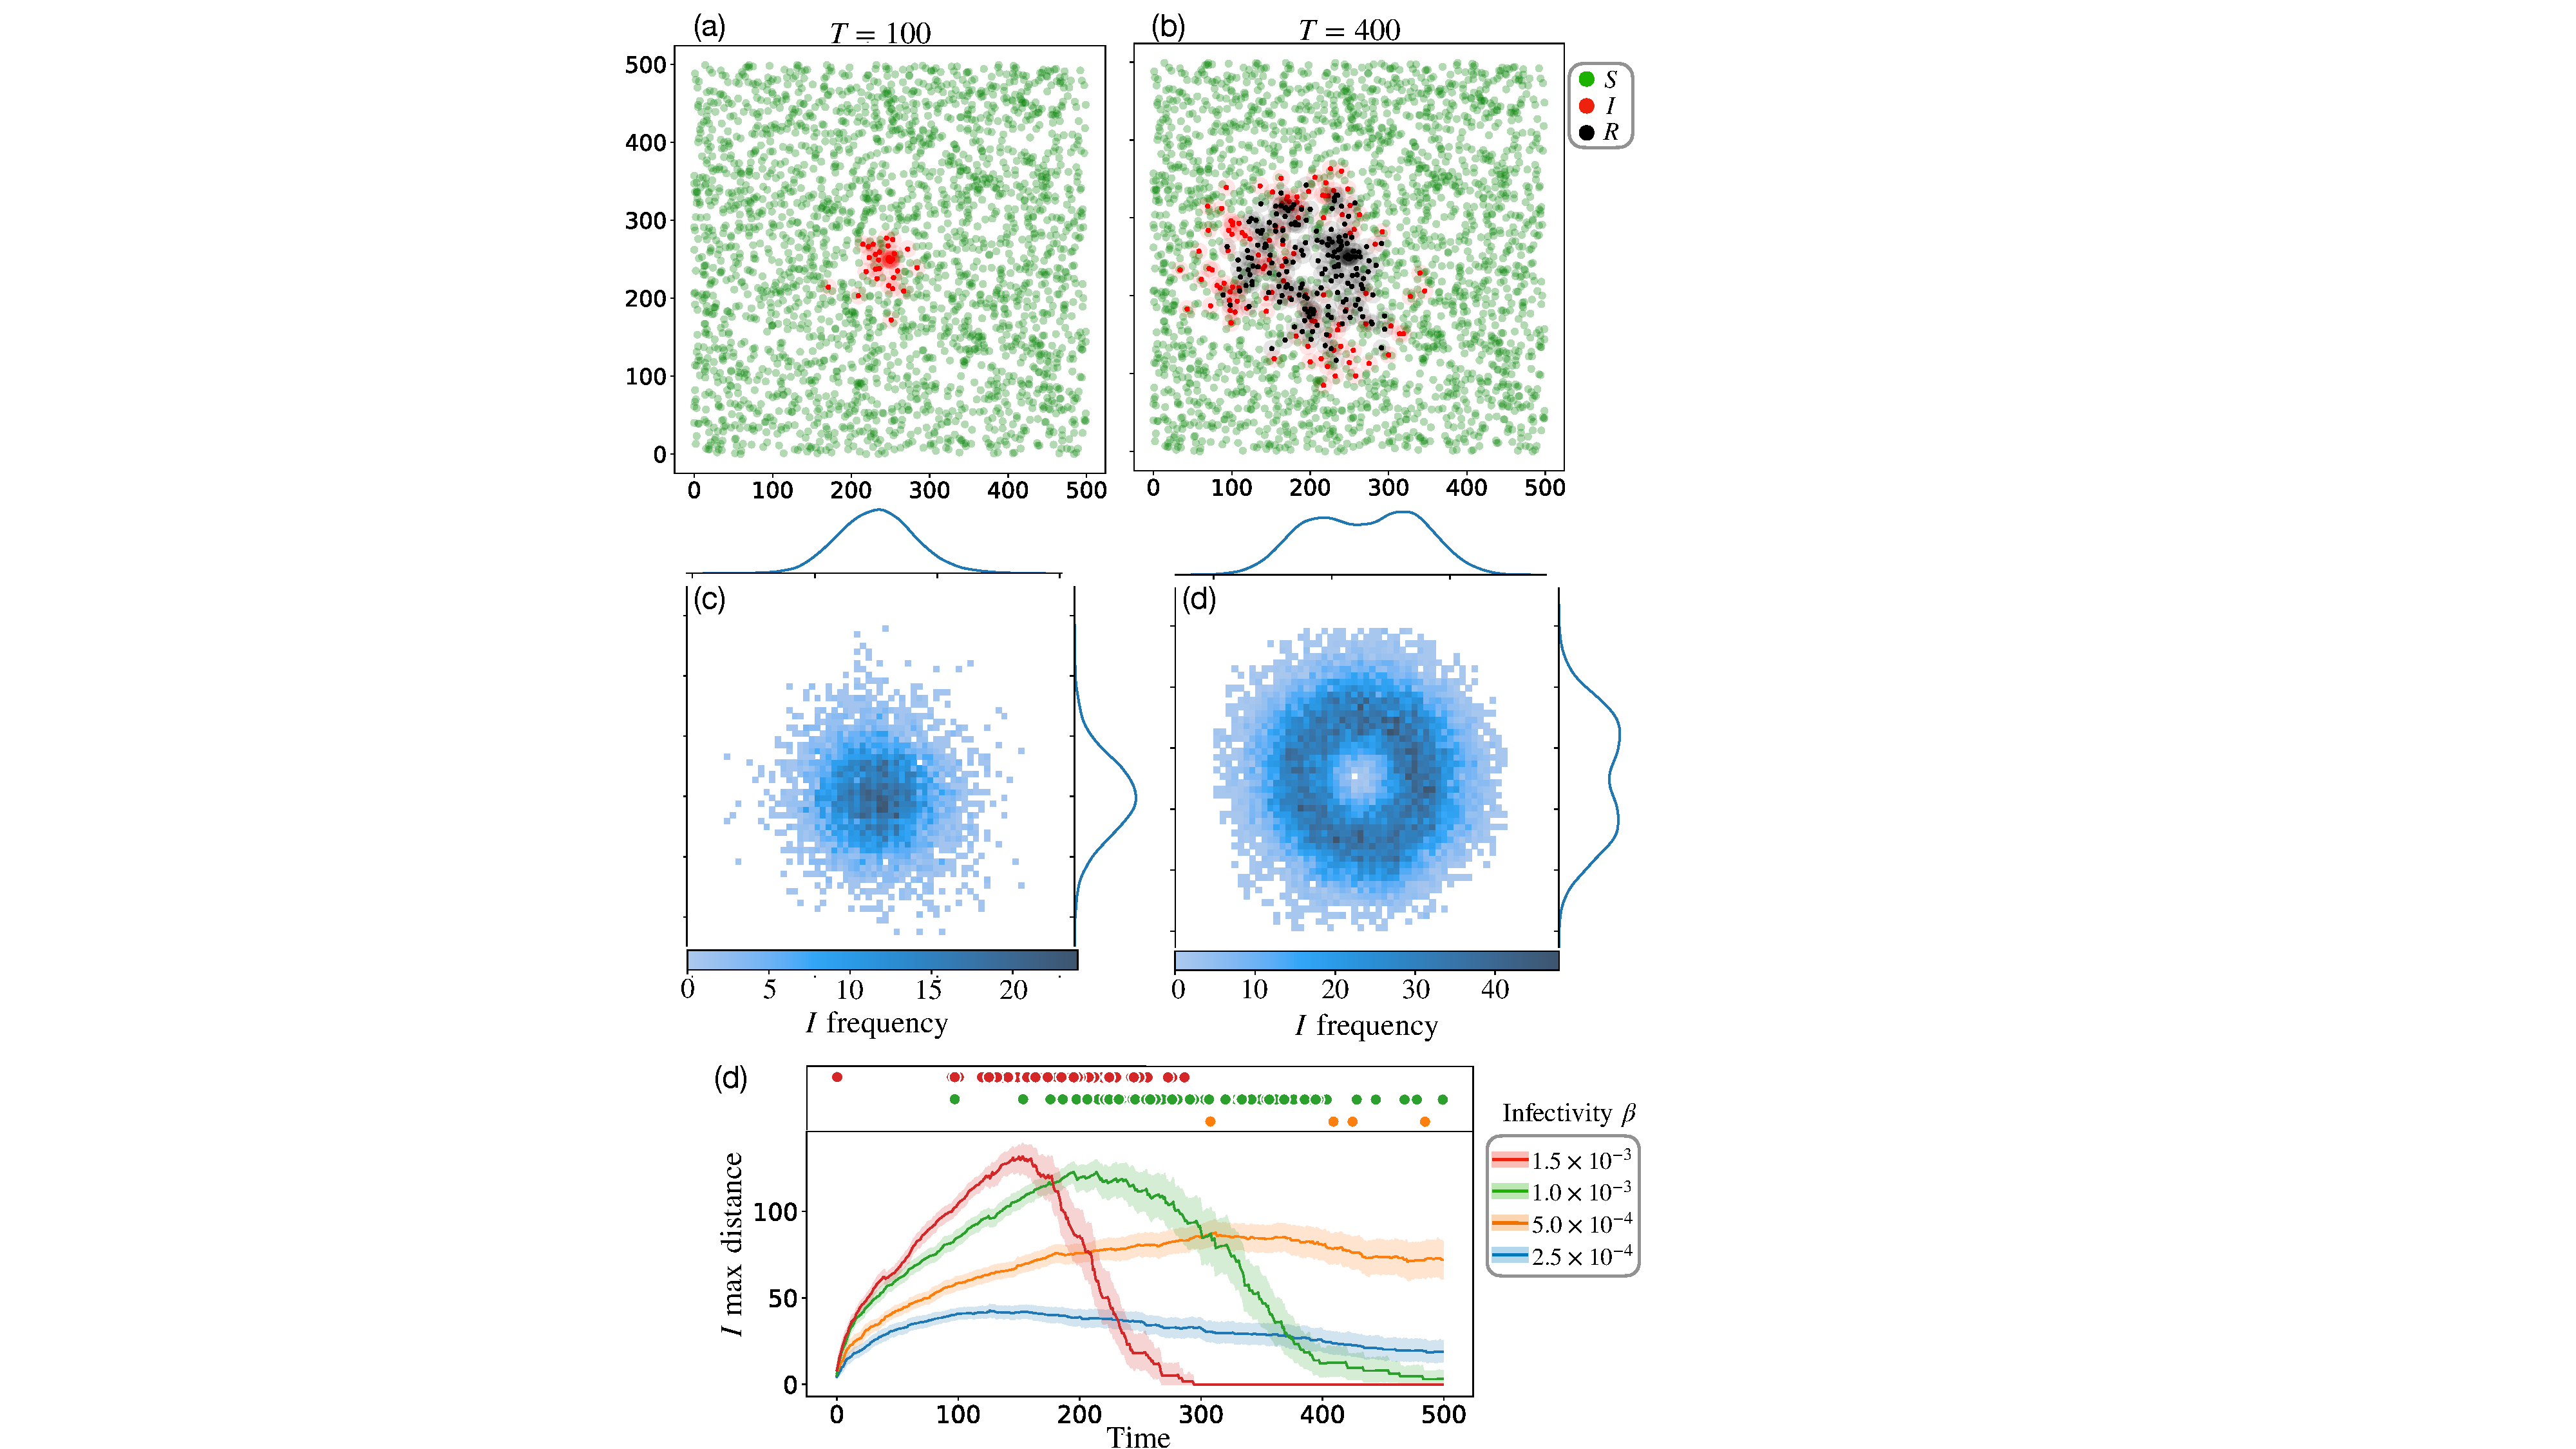
\includegraphics[scale=0.48]{chapter5/figures/fig1-sir-spatio-temporal.pdf}
    \caption{Percolation-like disease progression of the dispersal-based SIR model with a small dispersal length scale of $\ell = 25$. 
    All figures were accessed in a domain of size $\mathcal{L} \times \mathcal{L} = 500 \times 500$ and fixed host density $\rho=0.01$. (a-b) An evolving epidemic with infectivity $\beta=1.0\times 10^{-3}$ is shown through two time-steps. Green pixels represent susceptible trees in $S$, while red pixels represent infected trees at different steps in the $I$ category. Infected trees uniformly transition into the removed compartment at $t=100$, shown in black. (c-d) An ensemble-averaged spatio-temporal frequency distribution (of 200 repeats) representing the number of trees in the infected compartment. The probability of an infected tree located at row $x$ and column $y$ is represented by a kernel density estimate (ascertained via Seaborn, a statistical/plotting package in Python) in the upper and horizontal marginals. (d) The maximum infectious distance ensemble-averaged over 100 repeats for four infectivity parameters shown by colour.}
\label{fig:sgm-evol}
\end{figure}

After $t$ time steps, the maximum distance reached by the pathogen is $D_{max}(t)$.
Figure \ref{fig:sgm-evol}(e) shows the ensemble-averaged maximum infectious distance for four infectivity parameters, along with a $95\%$ confidence interval about the mean for each time step. The time-series data shown in Figure \ref{fig:sgm-evol}(e) indicates whether or not the pathogen dies off or survives to the domain boundary. Furthermore, scatter plots in the upper marginal of Figure \ref{fig:sgm-evol}(e) mark when the pathogen arrives at the domain boundary. A cluster of infectious-removed trees spans the domain whenever the pathogen survives long enough to propagate to the edge. 

Unsurprisingly, Figure \ref{fig:sgm-evol}(e) reveals that, on average, pathogens with higher infectivities propagate to the domain boundary quickest, illustrated by comparing the first (red) and second (green) highest infectivity line plots. In contrast, the lowest two infectivity values (blue and orange time series, respectively) fail to reach the domain boundary in most simulations, notwithstanding the small number of orange scatter points shown in the upper marginal.

Modelling the spread of disease for small $\frac{\ell}{\mathcal{L}}$ is helpful to understand the NLM and presents a clear connection to the percolation-based SLM. However, realistic dispersal-based tree disease is unlikely to exhibit slow marching travelling waves at these small spatial-scales. In particular, as $\frac{\ell}{\mathcal{L}}$ becomes larger, tracking the maximum distance inside a finite domain of size $L$ becomes ill-defined; undoubtedly this becomes even more relevant with fat-tailed dispersal kernels. Therefore, although the time-series $D_{max}(t)$ is justified for pathogen progression when $\frac{\ell}{\mathcal{L}}$ is small, an alternative metric is required to understand epidemic progression as we look to increase the scale of dispersal. Consequently, the reproductive ratio $R_0$ is introduced later in section \ref{sec:spatially-explicit-reproduction-ration}.


\subsection{Normalising infectivity $\beta$}

Before we move onward, a tool to fix epidemic impact over various dispersal length scales is outlined below.
Using $\beta$ to control infectivity in the model, as governed by equation \ref{eq:pr-dispersal-transition}, is pragmatic for single parameter of $\ell$\textemdash as shown in Figure \ref{fig:sgm-evol}.
However, suppose the dispersal parameter $\ell$ in equation \ref{eq:pr-dispersal-transition} is increased. 
Undoubtedly, a larger area under the unnormalised kernel, $\exp\big[-r^2/(2\ell^2)\big]$, would produce more secondary infections.
In turn, more secondary infections produced by each infected tree affords a more severe epidemic.
In this setup, infectivity, as defined in Equation \ref{eq:pr-dispersal-transition}, depends strongly on the scale of dispersal $\ell$ and epidemic-impact would vary significantly under different dispersal parameters.
Ideally, the infectivity (i.e the strength of interaction between trees) should not depend strongly on the dispersal kernel because this makes model comparisons over different length scales $\ell$ difficult. This motivates an updated scheme.

At the very least, $\beta$ could be manually varied to match the approximate epidemic-impact between different $\ell$ valued simulations\footnote{One may suggest that directly normalising the kernel poses a solution to fix the epidemic scale for all values of $\ell$.
Although, this is ultimately incorrect from an implementation perspective. 
If the Gaussian kernel in \ref{fig:sgm-evol} is normalised, it will cease to be a yield a probability describing individual tree-to-tree interactions and the transition between states.}. 
However, scaling $\beta$ differently for each $\ell$ parameter is cumbersome and ultimately untenable for many simulations.
A mathematical sleight-of-hand can resolve the dilemma by simply factoring out the dispersal normalisation from $\beta$:
\begin{equation}
    \beta = \frac{\beta^*}{2\pi\ell^2}
    \label{eq:normalised-infectivity}
\end{equation}
where $\beta^*$ is an `auxiliary' infectivity parameter that isolates infection pressure to a single parameter that remains fixed between simulations with different $\ell$ values.
In this manner, infectivity and the dispersal remain probabilities (i.e. $\beta=\beta^*/2\pi\ell^2 \in [0, 1]$, and $\exp\big[-r^2/(2\ell^2)\big] \in [0, 1]$ respectively), and epidemic severity will be matched between different $\ell$-valued simulations; the limitations of this method are discussed below in section \ref{sec:spatially-explicit-reproduction-ration}.
So, henceforth, unless otherwise stated, the remainder of this Chapter will employ the normalised infectivity.
That is, the right-hand side of equation \ref{eq:normalised-infectivity} will be substituted into equation \ref{eq:pr-dispersal-transition} (and the analytic expression of $R_0$ outlined below) to permit model comparisons over the parameter space of $\ell$.

\subsection{SIR fitting: dispersal-mediated contact-mixing}
\label{sec:SIR-fitting}

This section aims to shed light on whether or not the spatial NLM can recover a non-spatial process and if so, answer which parameter regime is required approximate the non-spatial process. Understanding when to include spatial dynamics becomes particularly important given the increased computational cost of spatial simulations. In a nutshell, why bother to include spatial dynamics if we could use a simpler non-spatial model? Consequently, we will fit the SIR model given by \cite{kermack-model} to simulated data from the NLM. Notwithstanding the spatially-structured host distribution, it makes sense to compare the NLM with predictions from the SIR framework given the same compartmental transitions $S \rightarrow I \rightarrow R$. 

Two parameters control the epidemic evolution in the SIR model, an infectivity rate $\beta$ and a removal rate $\gamma$. 
Both rates $\beta$ and $\gamma$ could be manually varied to match data from NLM simulations, though the task can be simplified significantly by considering $I$ as a function of $S$, accomplished as follows:
\[
\frac{dI}{dS}=\frac{dI / dt}{dS /dt}= \frac{\beta IS/N - \gamma I}{-\beta IS/N} = -1 + \frac{\gamma}{\beta} \frac{N}{S} \]
Letting $\alpha = \frac{\gamma}{\beta}$ we have:
\[
    dI = \Big(-1 + \frac{\alpha N}{S}\Big)dS
\]
Now using integration by separation of variables:
\begin{equation}
\label{eq:SIR-1param}
     I = -S + \alpha N \ln (S) + C
\end{equation}
where $C$ is a constant of integration. Thus, we have reduced the task of trying to match two parameters to considering a single one, namely $\alpha$. Before we can fit the NLM to equation \ref{eq:SIR-1param} we need to determine $C$. Initially $S_0 + I_0 + R_0= N$ and $R_0=0$ i.e. $R_0$ is the number of removed at $t=0$, not the reproductive ratio. Thus, evaluating equation \ref{eq:SIR-1param} at $t=0$ gives:
\begin{align*}
I_0 + S_0 & = N \alpha\ln (S_0) + C\\ 
 \implies C &= N - N \alpha \ln (S_0) 
\end{align*}
Upon substitution back into equation \ref{eq:SIR-1param} we have:
\begin{equation}
\label{eq:SIR-1param1}
    I = -S + N\big(1 + \alpha \ln (S/S_0)\big)
\end{equation}
more information on the behaviour of equation \ref{eq:SIR-1param} is given in the appendix \ref{A:sir-fitting}.
By fixing the initial conditions in the differential SIR equations to match the NLM simulations\textemdash i.e. with $I_0=1$ and $S_0=\rho \mathcal{L}^2$ \textemdash we can compare the NLM to the SIR model.

The canonical SIR model is non-spatial and rests on a `well-mixed' population assumption, as described in section \ref{ch2:lit-rev-compartmentalised-models}. In a well-mixed population, each individual is equally likely to make contact (or pass on the infection) with any other individual. Conversely, a spatially-structured dispersal-based model will generally not describe well-mixed contacts between individuals in the population because the infection probability decreases with distance\textemdash see \cite{cook2008constructing}. 

Nevertheless, we can expect an approximation to contact mixing when the scale of dispersal, set by $\ell$, becomes comparable to the domain. In this scenario, secondary infections are prone to disperse more uniformly over larger areas, in stark contrast to the localised (wave-like) transmission previously witnessed when $\ell$ is small. Hence, the comparisons below pay attention to the interplay of parameters $\ell$ and $\mathcal{L}$. Accordingly, Figure \ref{fig:SIR-fitting} shows the NLM fitted to equation \ref{eq:SIR-1param} for two domain sizes and two dispersal parameters.

Figure \ref{fig:SIR-fitting} contrasts SIR and NLM models. 
Ensemble-averaged data from the NLM is plotted in black and is shown alongside the 25 individual simulations in light blue. NLM simulations contrast the SIR model plotted in red. Tree density and infectivity in the NLM are fixed to $\rho=0.01$ and $\beta^*=4$, respectively. Notably, the parameters were large enough to ensure epidemics were witnessed in all simulations. Using least-squares\textemdash specially, the Levenberg-Marquardt algorithm \cite{more1978levenberg} implemented in Python\textemdash the ensemble mean was fitted to equation \ref{eq:SIR-1param}, shown in red. In all panels, the arrow of time is from right to left, i.e. initially, the number of trees in $S$ starts high and decreases as the number of trees in $I$ rises then falls.
 
 \begin{figure}
    \centering
    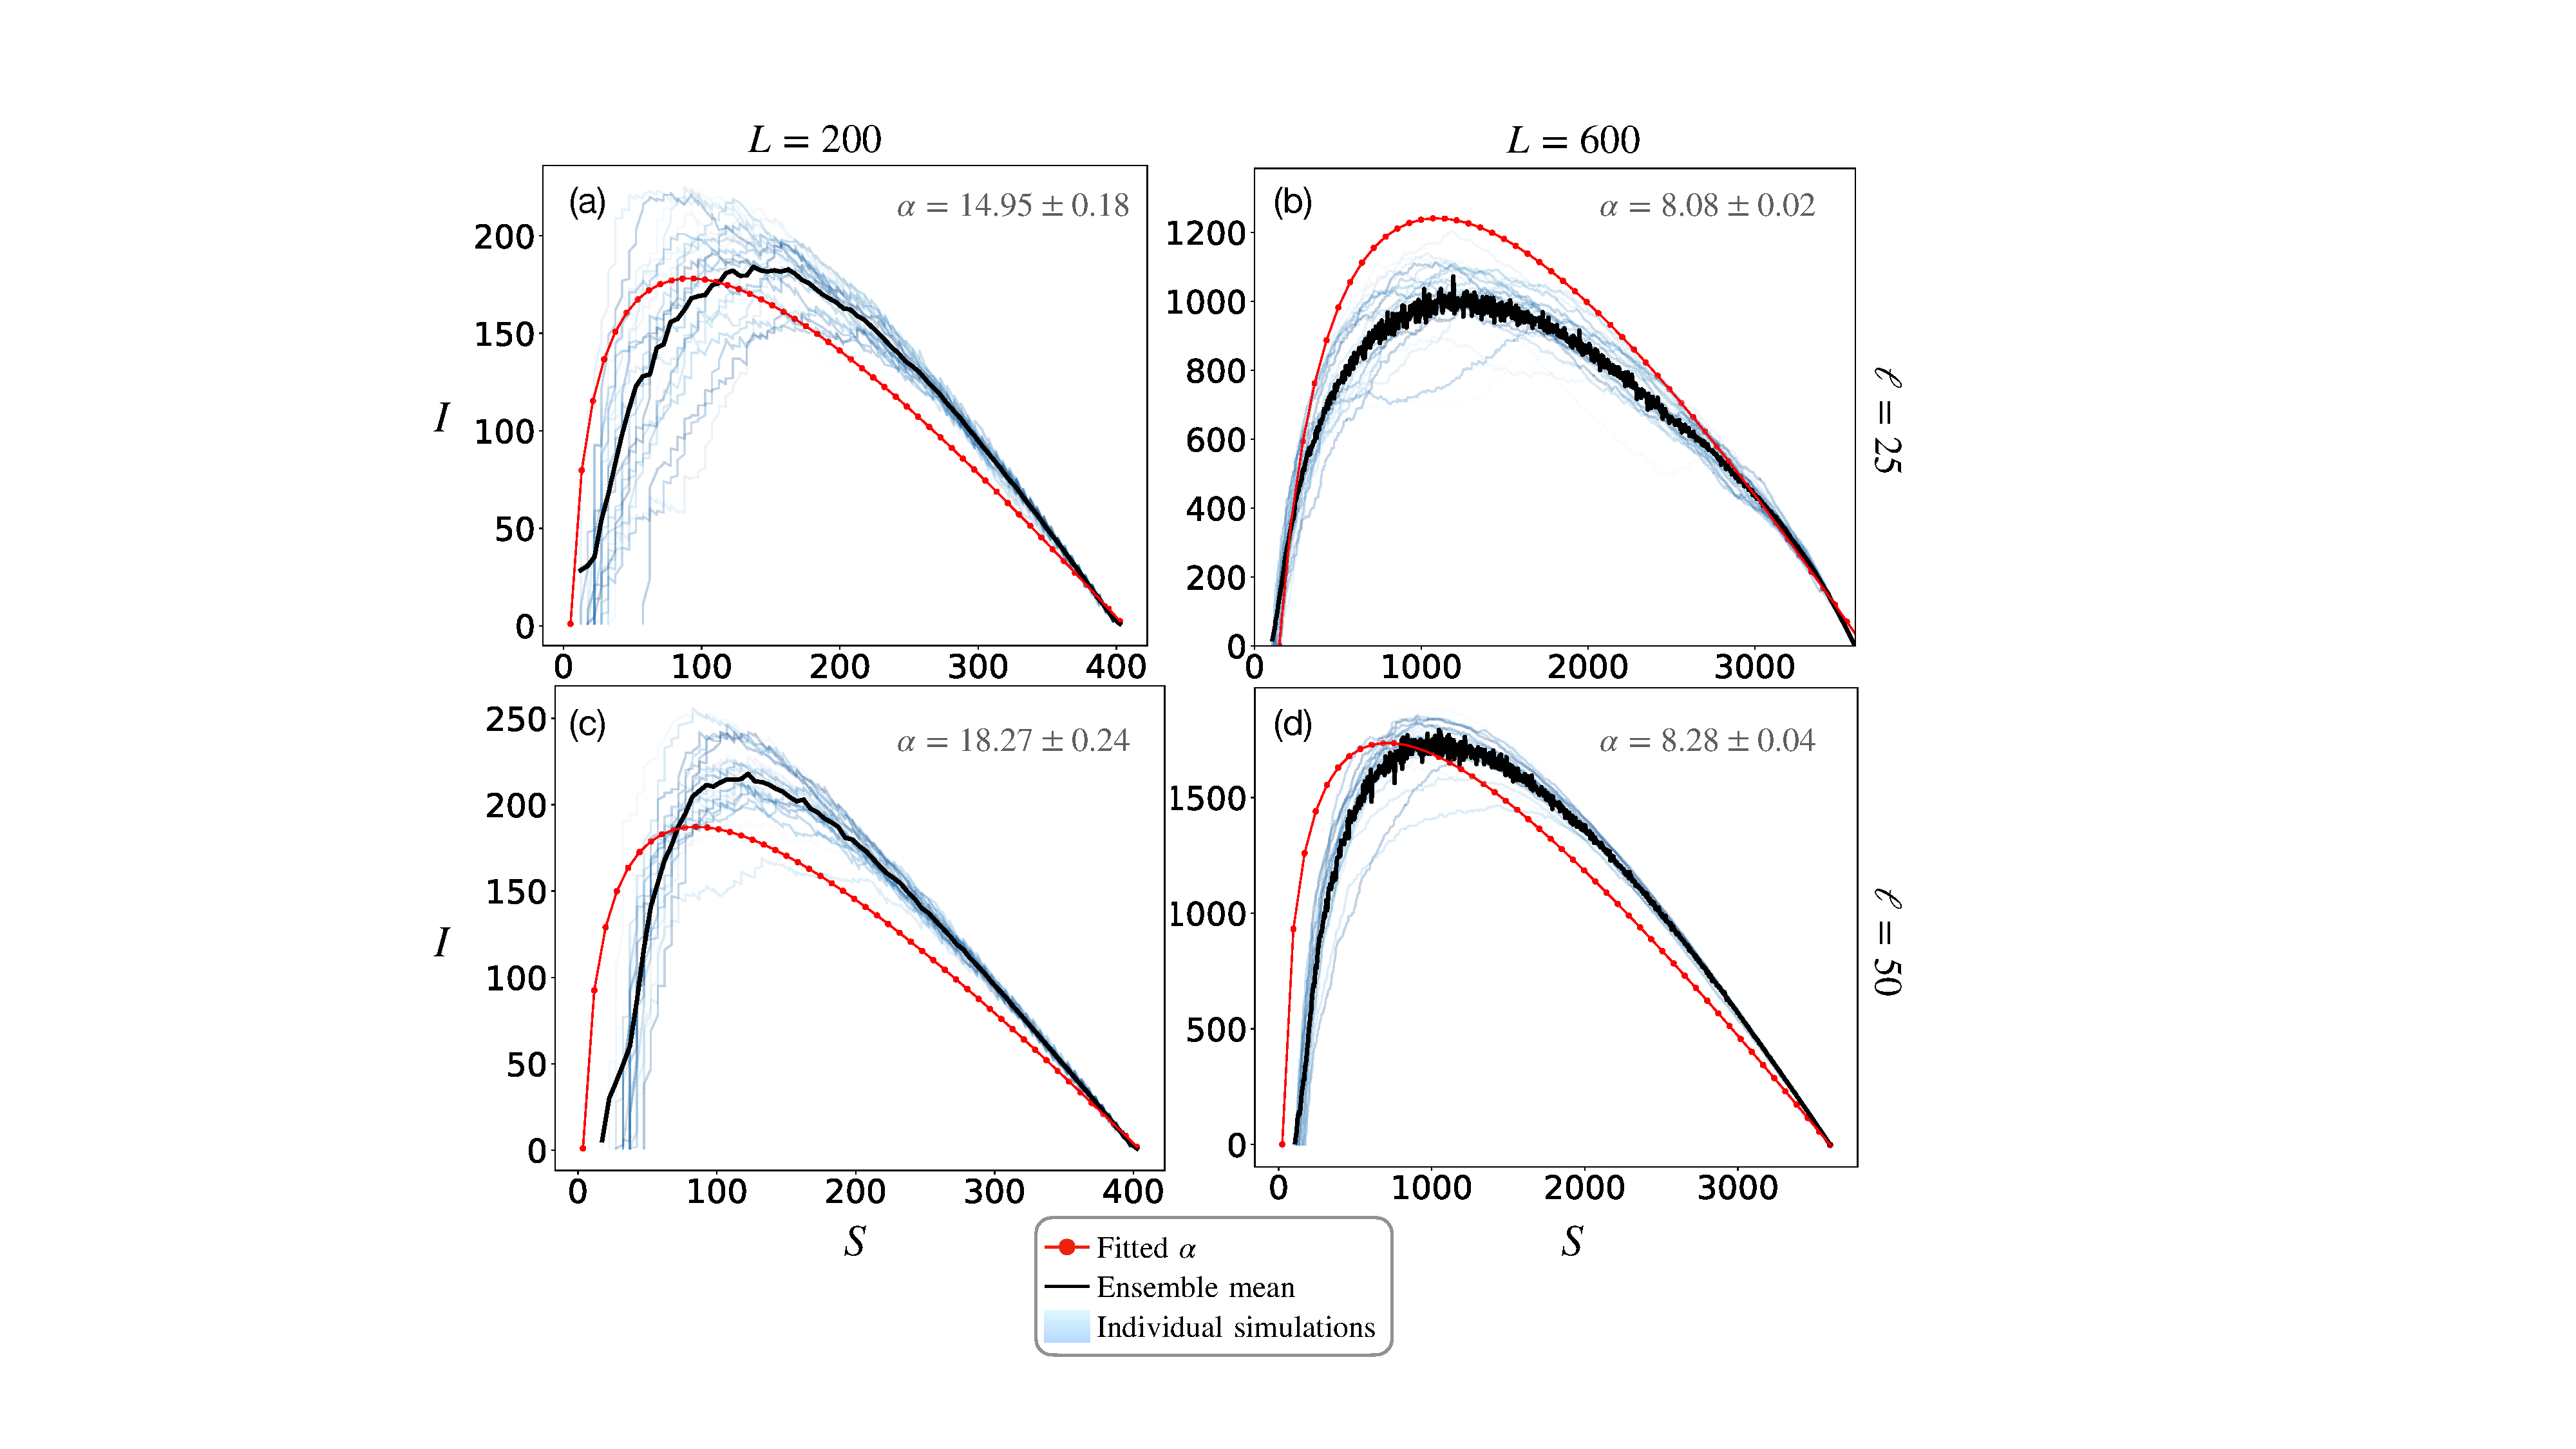
\includegraphics[scale=0.425]{chapter5/figures/fig2-sir-fitting-step.pdf}
    \caption{Fitting the non-local dispersal model (NLM) to the traditional SIR model given by \cite{kermack-model}. All simulations evolved with parameters $\beta^{*}=4$ and $\rho=0.01$ above the threshold for spread. (a) A small localised dispersal kernel of $\ell=25$ fitted against the canonical SIR. On a small domain of size $200\times 200$, the NLM spreads faster than the fitted SIR model. (b) On a larger patch of size $600\times 600$, the SIR model predicts a faster rate of spread in comparison to the NLM, illustrated by the disparity between red and black lines. (c) On $200\times 200$ sized domain, increasing the dispersal parameter to $\ell=50$ results in a similar trend to panel (b), albeit with slightly less agreement between NLM and SIR models. (d) Increasing the dispersal parameter to $\ell=50$ reduces the large disparity between SIR and NLM, shown in Figure (b).}
    \label{fig:SIR-fitting}
\end{figure}

Interestingly, for all but one panel in Figure \ref{fig:SIR-fitting}, epidemics progress faster in the NLM than predicted by the SIR model\textemdash indicated by the NLM having a steeper gradient beginning from $S_0=\rho\mathcal{L}^2$. 
One possible cause of disparity between models is due to infectious lifetime dynamics. 
Exponentially distributed lifetimes are implicit within the SIR model.
Whereas, the NLM relies on uniform transitions into the $R$ compartment that understood by examining Figure \ref{fig:SIR-fitting}(a), i.e. 400 hosts are present in the domain at time $t=0$ and it takes precisely $t=100$ steps to elapse before the first transition into $R$.

On the other hand, trees evolving with SIR dynamics will gradually transition into the $R$ compartment at all time steps according to an exponential distribution. 
For the same initial conditions, it follows that more infectious trees might be expected in the NLM between times $t\in [0, T]$, leading to more secondary infections that, on average, increase the scale of epidemic.
In appendix \ref{section:apendix_A}, Figure \ref{fig:SIR-fitting} is replicated, although equation \ref{eq:SIR-1param} was fitted to an exponentially distributed variant of the NLM.
Consequently, Figure \ref{fig:SIR-fitting-expontial} in appendix \ref{section:apendix_A} shows, a closer fit to equation \ref{eq:SIR-1param}.
 
Figure \ref{fig:SIR-fitting}(b) demonstrates another important aspect of NLM behaviour related to contact mixing in the spatial host distribution.
Looking at Figure \ref{fig:SIR-fitting}(b), a faster rate of spread is predicted for the SIR model,
demonstrated the divergence between red and black lines.
In this regime, $\frac{\ell}{\mathcal{L}}$ in the NLM is small, and contact-mixing in the host distribution can be assumed low \textemdash supported by Figure \ref{fig:sgm-evol} that demonstrated a wave-like spread. 
Moreover, the disparity between models is reduced by increasing the dispersal parameter to $\ell=50$, illustrated in Figure \ref{fig:SIR-fitting}(d).
Figure \ref{fig:SIR-fitting} therefore indicates that if the system is approximately well-mixed, the NLM spreads comparatively to the SIR, albeit slightly skewed because of uniform lifetime dynamics.
Whereas, if the system is not well-mixed, a slower epidemic marches across the domain in a wave-like manner that deviates significantly from the SIR model.
Altogether, these results point toward the inability of non-spatial models, such as the SIR model, to describe a spatially structured model of tree disease. That being said, in a parameter regime where the ratio $\ell / \mathcal{L}$ is sufficient for population mixing, the SIR model can describe the system with some accuracy\footnote{
Well-known results from percolation theory present a simple model analogy to the observations from Figure \ref{fig:SIR-fitting}.
Consider a large domain (of size $L$) below the percolation threshold, and sub-dividing the domain into boxes of size $\xi$, where $\xi / L$ is small.
Percolating clusters could be observed in each box i.e. at length scales comparable to $\xi$, but not $L$ see \cite{stauffer2018introduction} pages 64-65.}.


\section{A spatially-explicit reproduction number}
\label{sec:spatially-explicit-reproduction-ration}

As remarked earlier, percolation-based distance metrics become ill-defined when the pathogen can jump on long distances and a more robust metric is required to examine the model going forward.
As such, a basic reproduction number will be outlined for the NLM.
The concept of $R_0$ is widely used (and widely misinterpreted \cite{delamater2019complexity}),
and multiple methods of calculation exist in the literature \cite{perspectives-on-r0}.
Although, to recap, $R_0$ is fundamental to understand epidemic thresholds in human and animal populations. 

Crop-based reproduction ratios have been examined extensively
\cite{gubbins2000population, park2001invasion, doi:10.1146/annurev.phyto.011108.135838, van2011periodic},
yet the concept remains less explored in tree-based diseases. 
In general, $R_0$ is complicated, and may vary in response to numerous abiotic factors such as temperature, humidity and wind speed.
Notably, the threshold $R_0=1$ should separate regimes of epidemic and confinement for any definition of $R_0$.
Furthermore, when defining an $R_0$ value for tree-disease, the importance of spatial structure cannot be
ignored \cite{park2001invasion}.


\subsection{Approximating $R_0$ analytically}

In this section, an idealised, spatially explicit expression of $R_0$ is derived for the NLM. Defining an informative $R_0$-value for tree-based pathosystems is not simple, and care is needed when defining an $R_0$ value.  
The following thought experiment outlines an approach to approximate reproduction number:

\textit{Consider a single primary infected tree at time $t=0$, surrounded by a distribution of susceptible neighbouring trees. Throughout its infectious lifetime, the primary infection will lead to $R_0$ secondary infections. If secondary infections do not produce other tertiary infections, the neighbourhood around the primary infection remains untouched by other diseased trees, and the reproductive potential can be approximated by $R_0$.}

\begin{figure}
    \centering
    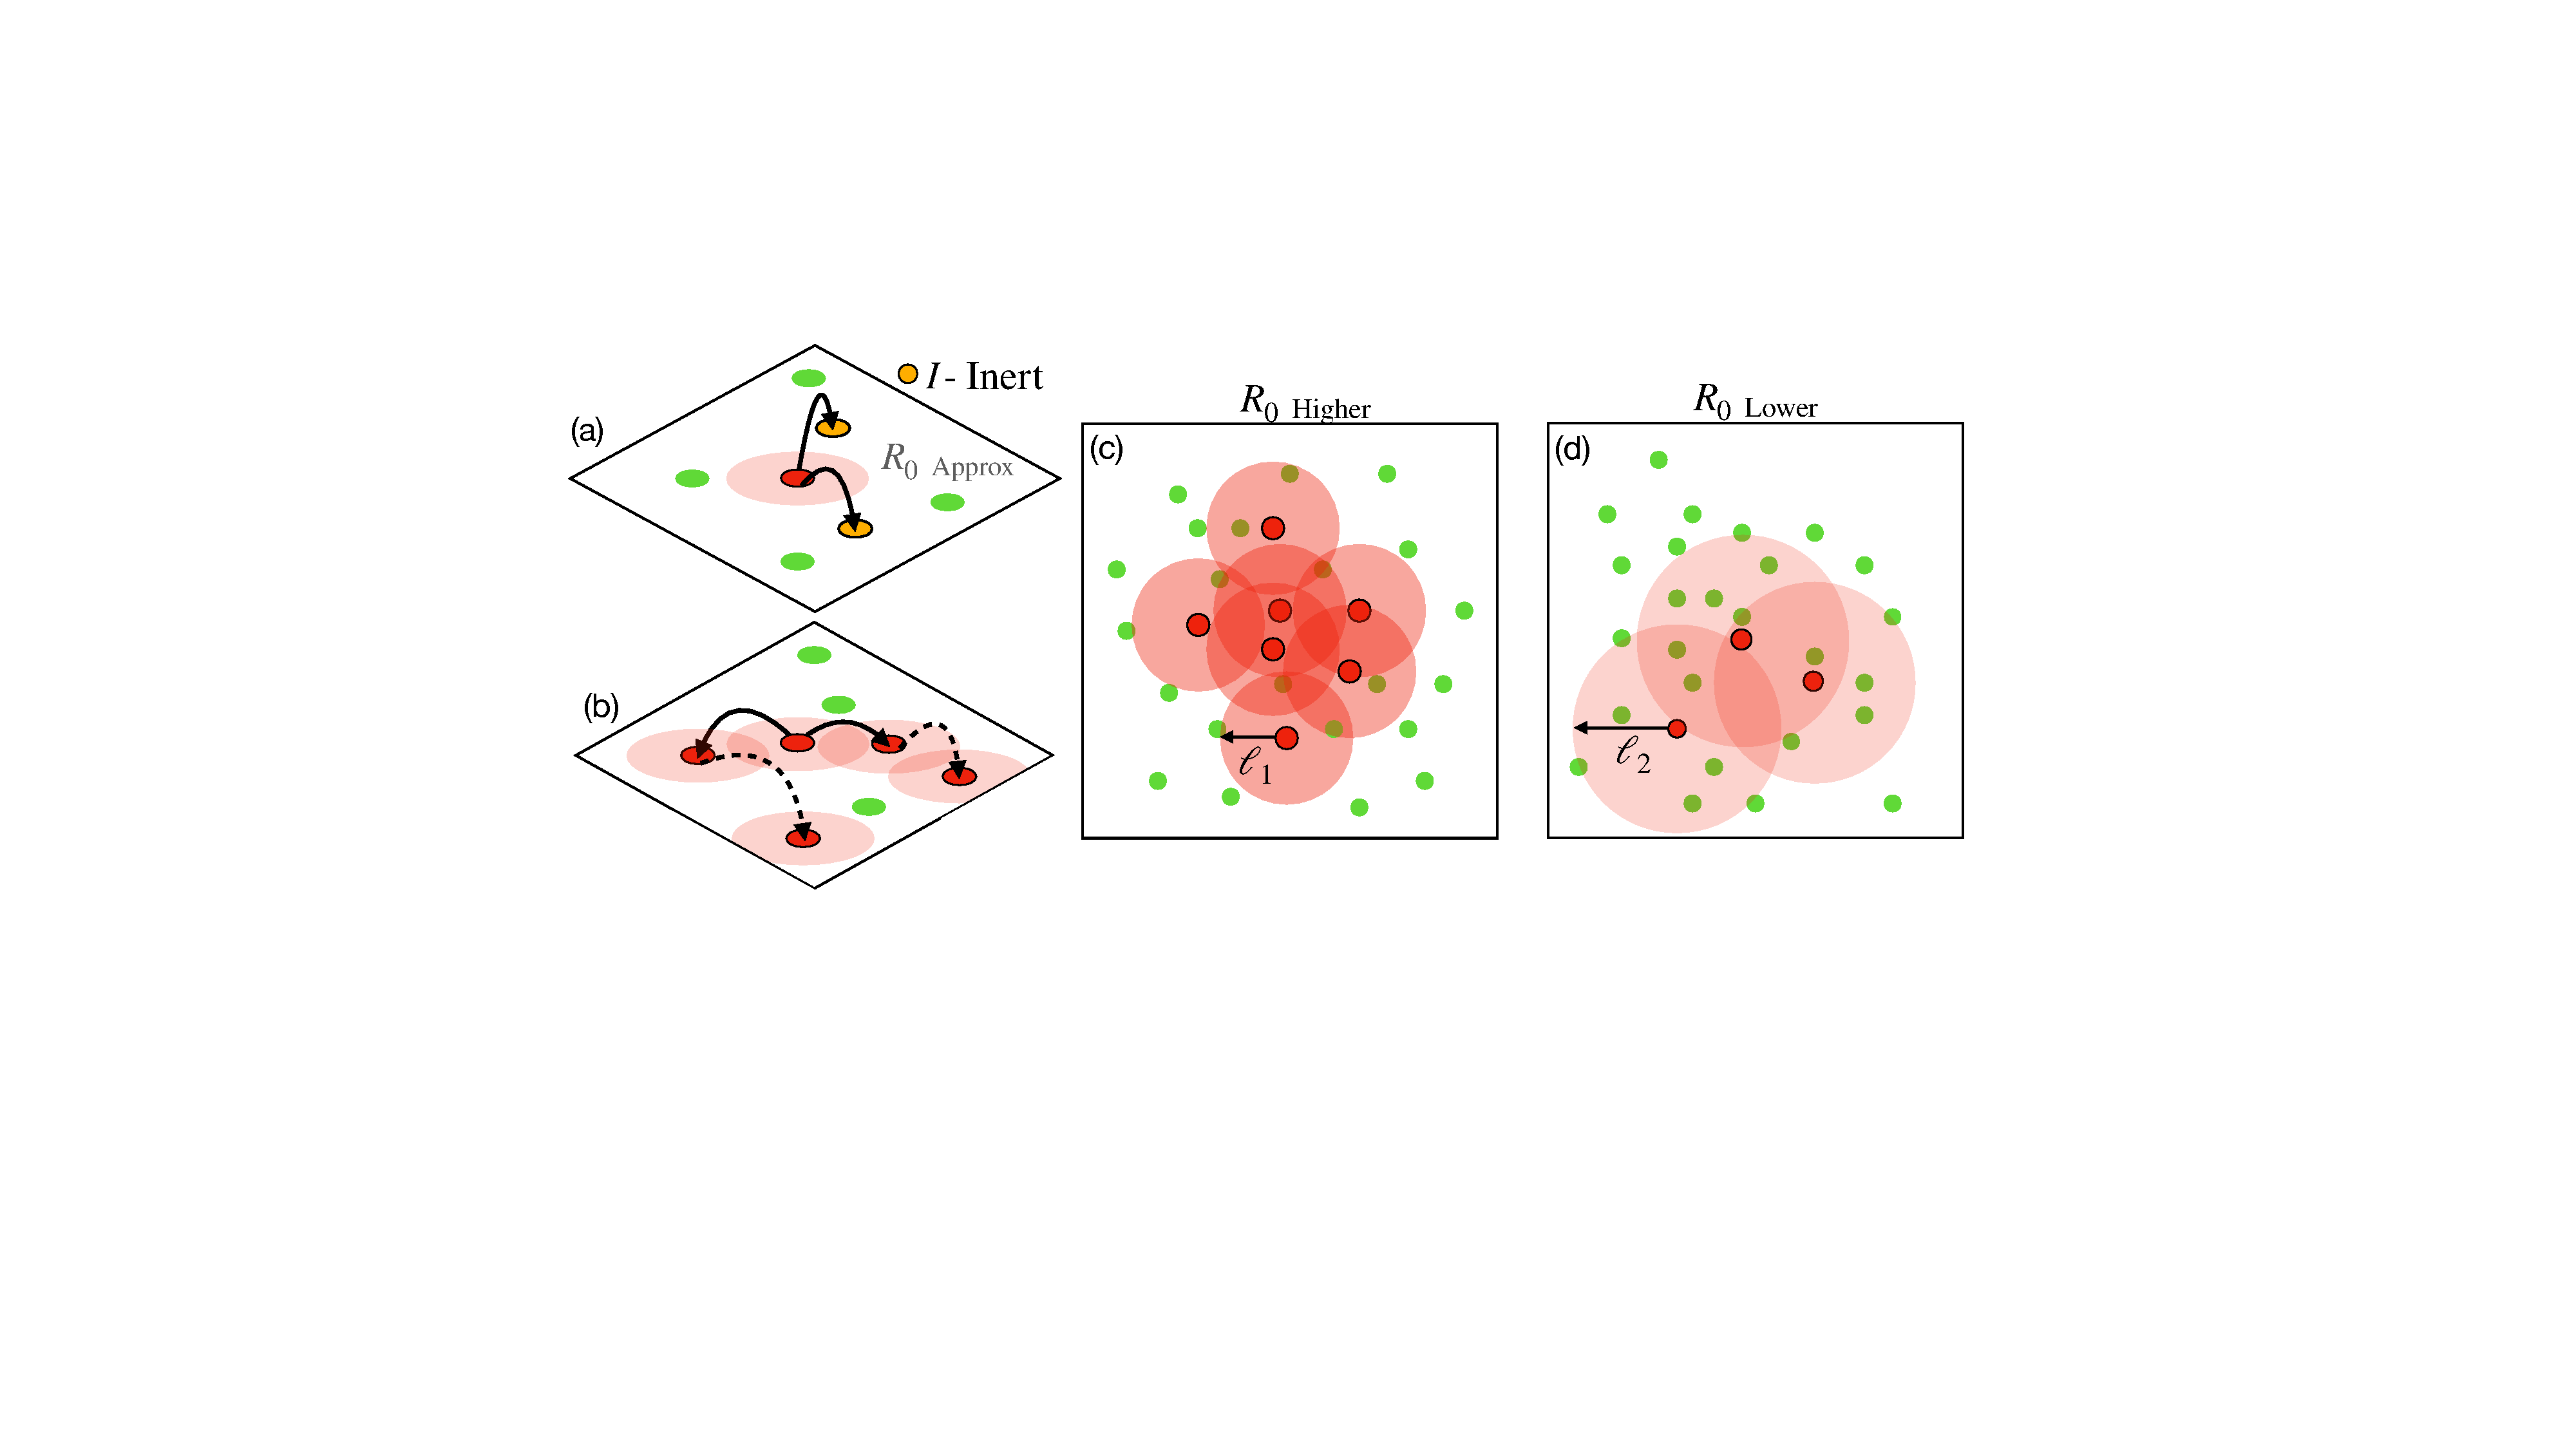
\includegraphics[scale=0.45]{chapter5/figures/fig3a-R0-approx.pdf}
    \caption{
    Approximating a spatially explicit value of $R_0$ as a function of $\rho$, $\beta$, $\ell$ and $T$.
    (a) An idealised scenario where secondary infections do not produce tertiary infections, but instead transition into an inert state\textemdash shown in amber.
    (b) The usual epidemic branching process where secondary infections produce tertiary (and so on) infections about the primary infection, shown by the solid and dashed arrows respectively.
    (c) Depictions of a highly infectious regime in the NLM, where $R_0$ is large and the dispersal parameter ($\ell_1$) is smaller.
    (d) Illustrations of an alternate, less invasive system when the scale of dispersal ($\ell_2$) happens to be larger. 
    The $R_0$ derivation aims to compute the scenario shown in (a), and becomes accurate in the epidemic regime illustrated in (d).
    }
    \label{fig:R0-approx}
\end{figure}

The thought experiment simplifies the epidemic branching process by neglecting tertiary (quaternary, and so on) infections,
illustrated by comparing Figures \ref{fig:R0-approx}(a-b). In turn, simplifying the system will help keep the mathematics tractable and permit an analytic derivation of $R_0$ without advanced mathematics. However, the derivation will be idealised and likely to overestimate the actual reproduction ratio in specific epidemic regimes.

Figures \ref{fig:R0-approx}(c-d) illustrate two hypothetical epidemic systems, with higher and lower $R_0$ values.
When the scale of dispersal is smaller (but still larger than the average distance between trees) and infectivity is high, as in Figure \ref{fig:R0-approx}(c), we expect a coupled system with a large number of secondary infectious induced inside a smaller area. In this case, the $R_0$ approximation would deviate from model simulations because secondary/tertiary infections would reduce the host density about the primary infection.
In other words, the finite-sized population gives rise to negative spatial correlations when other infected trees reduce the local density of susceptible hosts. The reader is referred to \cite{R0-perc-ref} for a helpful discussion of $R_0$, heterogeneity, spatial correlations and finite-size effects.

Conversely, Figure \ref{fig:R0-approx}(d) depicts a scenario when the pathogen induces a lower number of secondary infectious over a larger area. Hence, in the limit where secondary/tertiary infected trees do not influence the local density around the primary infection, the thought experiment (mentioned above) is expected to become increasingly accurate. 
However, even with a larger dispersal kernel, the approximation illustrated by Figure \ref{fig:R0-approx}(a) would become more inaccurate for highly invasive systems with a large $R_0$. 

For example, incredibly high values $R_0\in [30, 70]$ have been estimated for wheat stripe rust (WSR) epidemics \cite{severns2019consequences, mikaberidze2016invasiveness}. Nevertheless, 
a field of crops is significantly dense in comparison to an average tree population distributed over the landscape\textemdash discussed extensively in section \ref{sec:ch4-discussion} concerning oak. Consequently, we argue that, in general, the reproduction ratio of a tree pathogen is unlikely to reach super epidemic regimes that parallel WSR epidemics; supported further by estimates of $1 \lessapprox R_0 \lessapprox 6$ for the Dutch elm disease epidemic in GB \cite{swinton1996dutch} and $1 \lessapprox R_0 \lessapprox 4$ for oak processionary moth epidemics in London \cite{wadkin2022inference}.

\subsection{Derivation}

Suppose the domain is uniform with density $\rho_0$ at time $t=0$, and one singular infected tree exists inside a large domain.
In such a configuration, the mean number of secondary infections expected over the first time-step can be calculated by integrating equation \ref{eq:pr-dispersal-transition} as follows:
\begin{equation}
    R_0(t = 0) = \beta \rho_0 \int^{\infty}_{-\infty} \exp\Big(-\frac{r^2}{2\ell^2}\Big)dr= 2\pi\beta\rho_0\ell^2
\end{equation}
If host (re-)growth is neglected, less trees are available to infect at time-step $t+1$. 
Tree density can therefore be seen as a monotonically decreasing function of time $\rho(t)$, leading to the expression:
\begin{equation}
    R_0(t) = 2\pi\beta\ell^2\rho(t)
    \label{eq:r0-A}
\end{equation}
this expression presents a convenient relationship between tree density and the number of expected secondary infections. 
In a large but finite domain, of size $\mathcal{L}$, tree density approximately follows:
\begin{equation}
\label{eq:drho/dt}
    \frac{d\rho}{dt} = - \frac{R_0(t)}{\mathcal{L}^2} = -\frac{2\pi\beta\ell^2\rho(t)}{\mathcal{L}^2}
\end{equation}
Solving the above, with initial condition $\rho_0$ at $t=0$, leads to:
\begin{equation}
\label{eq:rho(t)-linear}
    \rho(t) = \rho_0 \exp\Big(-\frac{2\pi\beta\ell^2}{\mathcal{L}^2} t \Big)
\end{equation}
If density reductions from other secondary and tertiary infections are neglected, the final number of expected secondary infections after $T$ infectious time-steps is given by:

\begin{equation}
\label{eq:Appendix_final_r0_approx}
    R_0(T) =  \mathcal{L}^2\big(\rho_0 - \rho(T)\big) = \mathcal{L}^2\rho_0\Big[1 - \exp\big(-\frac{2\pi\beta\ell^2}{\mathcal{L}^2} T \big) \Big]
\end{equation}

Equation \ref{eq:Appendix_final_r0_approx} can be used as a first approximation toward an $R_0$ value\textemdash the reader can find an equivalent, discrete-time derivation in Appendix \ref{eq:alternate-R0}.
Nonetheless, uniform density reductions (in equation \ref{eq:drho/dt}) assume that secondary infections are equally likely at all spatial locations about the primarily infected tree. 
On average, neglecting spatial variations overestimates the number of secondary infections induced by the tail-ends of the dispersal kernel,
thus giving rise to a greater $R_0$ value.
A more accurate, albeit more complex, equation can be derived, allowing for Gaussian spatial variations

For transparency, the above derivation is solely based on $\beta$, and not the normalised infectivity parameter. 
However, from the exponential exponent in equation \ref{eq:Appendix_final_r0_approx}, it is clear to see how normalising the infectivity ($\beta^*/2\pi\ell^2$) prevents
the number of expected secondary infections dependency on $\ell$. That is, substituting $\beta^*/2\pi\ell^2$ into the equation \ref{eq:Appendix_final_r0_approx} leads to an exponent, (i.e. $T\beta^*/L^2$) independent of $\ell$.

\subsubsection{Incorporating Gaussian dispersal}

\label{sec:r0-derivation}
Equation \ref{eq:Appendix_final_r0_approx} neglects a spatially varying transmission probability, 
though it can be refactored by first re-writing the density as:
\begin{equation}
\label{eq:rho(t)-ga-variations}
    \rho(r, T) = \rho_0\exp \big(-\beta T g(r; \ell) \big)
\end{equation}
where $g(r;\ell)$ is a Gaussian kernel. 
Equation \ref{eq:rho(t)-ga-variations} can be interpreted as the generalised form of equation \ref{eq:rho(t)-linear}, this time incorporating Gaussian spatial variations into $R_0$.
Upon substitution back into equation (\ref{eq:Appendix_final_r0_approx}), the total number of secondary infections after $T$ time-steps is given by:

\begin{equation}
\label{eq;R0(t)-ga-variations}
   R_0(T) = \int ^\infty _0 2\pi r \big (\rho_0 - \rho(r, T)\big)dr =  \int ^\infty _0 2\pi r \rho_0 \Big[1 - \exp\big(-\beta T g(r;\ell)\big) \Big]dr
\end{equation}

Note, the finite lattice square of size $\mathcal{L}^2$ has been replaced with integration in polar coordinates over $dr$. 
Equation \ref{eq;R0(t)-ga-variations} is hard to solve directly, but it can be integrated by performing a series expansion on the exponential term. 
One may then proceed to integrate on a term-by-term basis:

\begin{equation} 
\label{eq:Appendix_final_expression}
\begin{split}
R_0(T) & = \int^\infty_0 2\pi r \rho_0 \Big[1 - \exp \big( -\beta T g(r;\ell)\big)\Big]dr \\
& = 2\pi\rho_0 \int^\infty _0 r \Big[1 - \sum^\infty_{n=0} \frac{\big(-\beta T)^n}{n!} \exp\big(-\frac{r^2}{2\ell^2}\big)^n  \Big] dr \\
& = 2\pi\rho_0 \int^\infty _0 r \Big[\sum^\infty_{n=1} \frac{(-1)^{n+1}\big(\beta T)^n}{n!} \Big(\exp(-\frac{n r^2}{2\ell^2} ) \Big)  \Big] dr \\
& = 2\pi\rho_0 \sum^{\infty}_{n=1} \frac{(-1)^{n+1} (\beta T)^n}{n!} \int^\infty _0 r \exp(-\frac{n r^2}{2\ell^2})dr  \\
& = 2\pi\rho_0 \ell^2 \sum^{\infty}_{n=1} \frac{(-1)^{n+1}(\beta T)^n}{(n)(n!) }
\end{split}
\end{equation}

if $\beta$ and $T$ are small, the $1^{st}$ order term in equation \ref{eq:Appendix_final_expression} is sufficient to approximate $R_0$ as a linear function of $T$\textemdash
confirmed by numerical simulations in the next section. 
Finally, equation \ref{eq:Appendix_final_expression} can be summed to give:
\begin{equation} 
\label{eq:Appendix_final_expression1}
\begin{split}
R_0(T) & = 2\pi\rho_0 \ell^2 \sum^{\infty}_{n=1} \frac{(-1)^{n+1} (\beta T)^n}{(n)(n!)}\\
& =  2\pi\rho_0 \ell^2 \big(E_1(\beta T) + \ln (\beta T) + \gamma\big)
\end{split}
\end{equation}
where the function $E_1(x)$ is the mathematically well studied exponential function $E_1(x)=\int^{\infty}_x t^{-1}\exp^{-t}dt$ and $\gamma$ is the Euler–Mascheroni constant $\approx 0.57721$.
Intriguingly, the jump between equations \ref{eq:Appendix_final_expression} and \ref{eq:Appendix_final_expression1} is well known in the field of complex analysis\textemdash see \cite{abramowitz1948handbook}, page 228.
Alternatively, the summation in equation \ref{eq:Appendix_final_expression} could equivalently be given as:
\begin{equation}
\label{eq:ein}
     \mathrm{Ein}(\beta T) = \sum^{\infty}_{n=1} \frac{(-1)^{n+1} (\beta T)^n}{(n)(n!)}
\end{equation}
where $\mathrm{Ein}$ is known as the `entire' function, leading to the well established relation:
\[
E_1(z) = -\gamma - \ln(z) + \mathrm{Ein}(z)
\]
The next section will investigate the suitability of \ref{eq:Appendix_final_expression1} to describe the NLM.

\section{$R_0$ behaviour: analytics vs numerics}

% R0 can be calculated from experimental data : \cite{segarra2001epidemic}
% \label{ch5:dispersal-model}
\begin{figure}
    \centering
    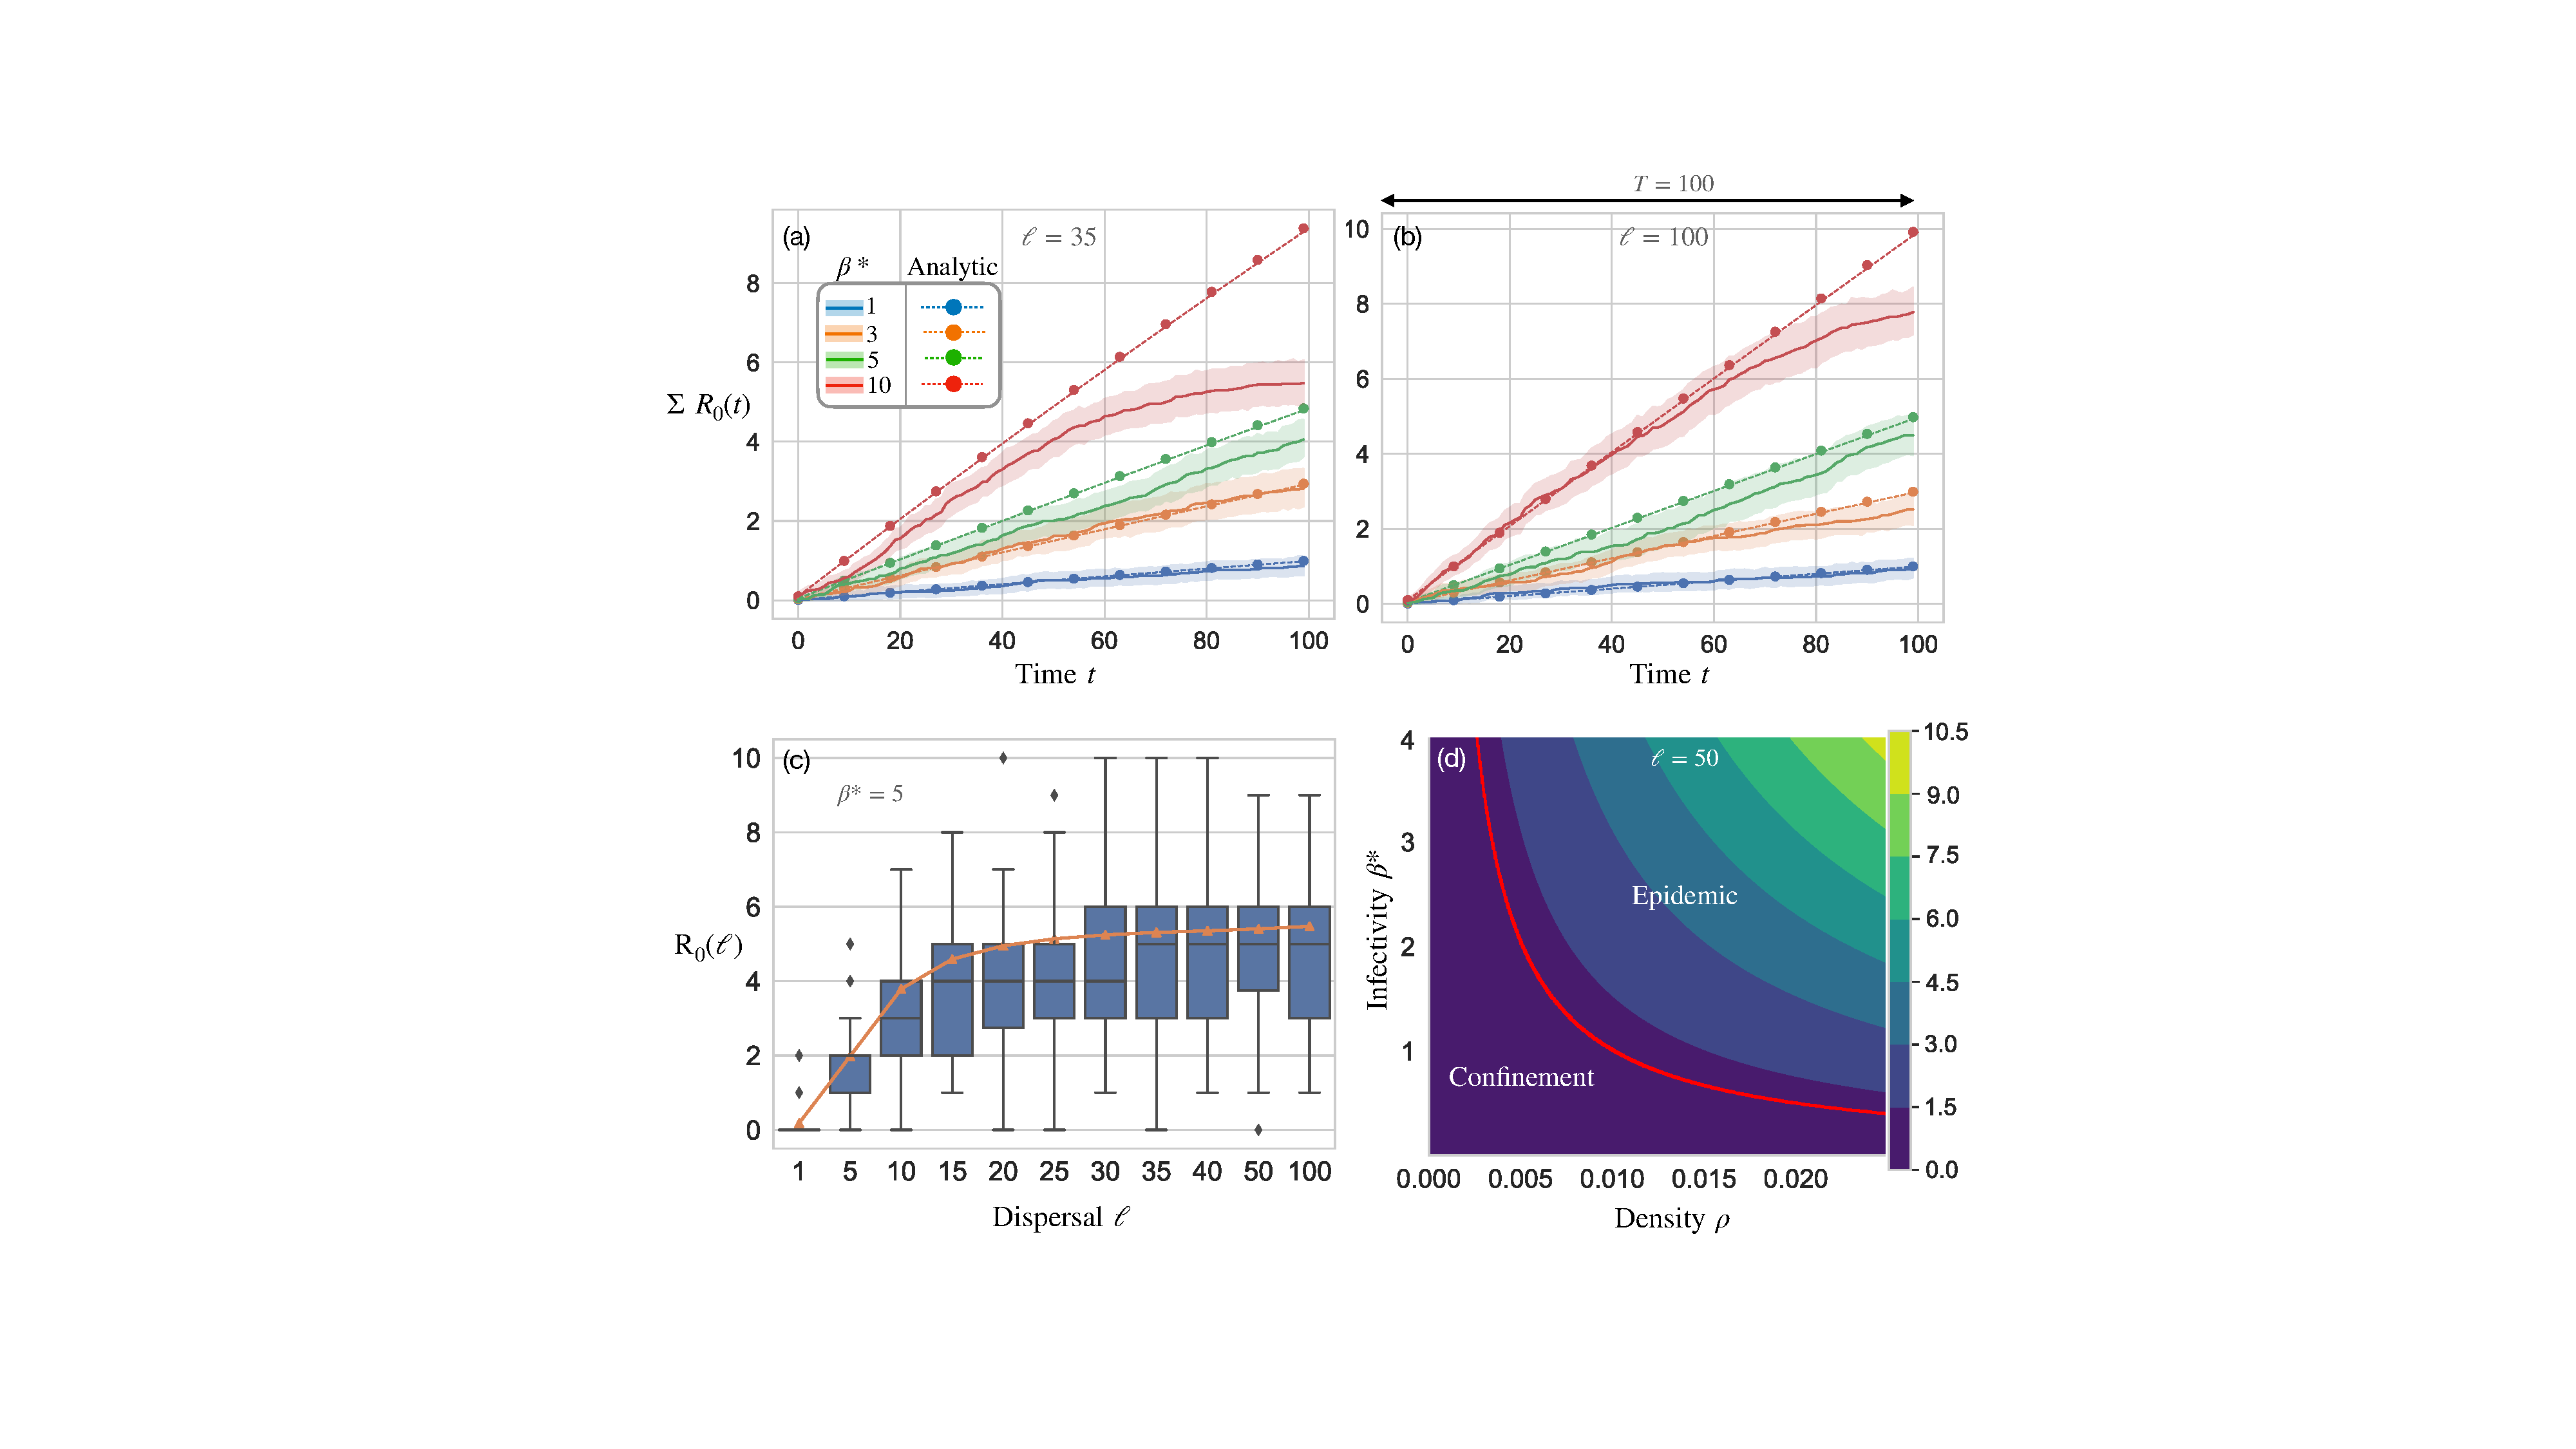
\includegraphics[scale=0.475]{chapter5/figures/fig3b-R0-analytic.pdf}
    \caption{Comparisons between the analytical expression for $R_0$, according to equation \ref{eq:Appendix_final_expression1}, and numerical simulations.
    In panels (a-b), The cumulative sum of secondary infections are ensemble-averaged (50 repeats) over the infectious lifetime of $T=100$ steps.
    (a) When the scale of dispersal is smaller ($\ell=35$), a high infectivity (in red) causes $R_0$ to saturate to a maximum over the infectious period.
    For smaller infectivities (blue-green), $R_0$ increases at a constant rate and fails to saturate.
    (b) For a larger dispersal kernel ($\ell=100$) and high infectivity, $R_0$ increases at a more constant rate, 
    yet deviations still exist at the conclusion of its infectious lifetime.
    (c) $R_0$ is shown as a function of the dispersal parameter for fixed infectivity $\beta^*=5$. For small length scales, the normalised infectivity produces a less infectious outbreak. However, $R_0$ is approximately fixed for larger $\ell$ values. Analytic predictions, shown in orange, tend to overestimate the spread for small $\ell$.
    (d) The 2D $R_0$ phase plane predicted by equation \ref{eq:Appendix_final_expression1}. A threshold, given by $R_0=1$, is plotted in red that predicts the separation between confinement and epidemic.}
    \label{fig:R0-analytic-vs-sims}
\end{figure}

In Figure \ref{fig:R0-analytic-vs-sims}, the analytic predictions of $R_0$ from equation \ref{eq:Appendix_final_expression1} are compared against numerical simulations. 
Figures \ref{fig:R0-analytic-vs-sims}(a-b) plot the total number of secondary infections due to the primary infection over its lifetime, denoted by $\sum_{t=0}^T R_0(t)$.
In both panels (a-b), NLM simulations were ensemble-averaged $N=50$ times for four infectivity values, indicated by the solid coloured lines. 
The final value of $R_0$ is observed when the infectious lifetime of $T=100$ steps is concluded.
Figures \ref{fig:R0-analytic-vs-sims}(a-b) show two epidemic scenarios, with lower ($\ell=35$) and higher ($\ell=100$) dispersal parameters.
As expected, equation \ref{eq:Appendix_final_expression1} tends to overestimate $R_0$ for both dispersal parameters when infectivity is high, illustrated by the dotted scatter plot.

The time-series in Figure \ref{fig:R0-vs-NLM-sims}(a) reveals that lower $\beta^*$ parameters produce a constant infection rate, indicated by linear relationship in blue-green.
Equation \ref{eq:Appendix_final_expression1} agrees well with these lower infectivity parameters. However, large deviations from model output can be seen for $\beta^*=10$ at later times. 
Here, the number of new secondary infections plateau for $\beta^*=10$ because other secondary/tertiary infections reduce host density around the primary infection. Subsequently, at later times, fewer and fewer trees in the primary infections neighbourhood are available to infect, causing $R_0$ to level off.
Thus, equation \ref{eq:Appendix_final_expression1} describes constant transition rates accurately but deviates from model simulations when infection rates decrease because other (secondary/tertiary) infections reduce host local densities.

In Figure \ref{fig:R0-vs-NLM-sims}(b), the dispersal parameter is increased to $\ell=100$.
A larger dispersal kernel encompasses a larger neighbourhood.
Subsequently, $R_0(t)$ saturates less for higher $R_0$ values, in contrast to Figure \ref{fig:R0-vs-NLM-sims}(a).
Despite a surprising degree of simplicity, the linear relation for lower $\beta^*$ parameters is predicted by equation \ref{eq:Appendix_final_expression1}.
The linearity can be understood by noting that when $\mathrm{Ein}(\beta T)$ is small in comparison to $\ell^2$ (and $\beta T$ is small), the first-order term inside equation \ref{eq:Appendix_final_expression1} reduces to a linear equation in $T$.
More interestingly, however, we can observe that $R_0$ is similar when $\beta^*$ is low, revealed by comparing the blue-green lines in Figures \ref{fig:R0-vs-NLM-sims}(a-b).
Whereas, for higher infectivities, $R_0$ tends toward a smaller value in Figure \ref{fig:R0-vs-NLM-sims}(a) comparison to panel (b).
Observing $R_0$ deviate with different $\ell$ parameters compels a study of $R_0$ over the space of $\ell$, which leads to Figure \ref{fig:R0-vs-NLM-sims}(c).

In Figure \ref{fig:R0-vs-NLM-sims}(c), the basic reproduction number $R_0$ is assessed over a range of dispersal kernels.
Tree density in Figure \ref{fig:R0-vs-NLM-sims}(c) is fixed fixed to $\rho=0.01$ together with infectivity $\beta^*=5$.
Predictions from equation \ref{eq:Appendix_final_expression1} are shown in orange,
and $R_0$ can be seen to increase with the dispersal kernel up to around $\ell \in [25, 30]$ before saturating to $R_0 \sim 5$. 
When $\ell$ is small, $R_0$ is low; the reason for this are two-fold: 
(A) neighbourhoods defined by a small $\ell$ parameter are likely to become fully occupied by secondary-infected trees
(B) the scale of dispersal is less than the average distance between trees, thereby preventing the spread.
Then, as the kernel is increased, $R_0$ asymptotically increases to a maximum value beyond which increasing $\ell$ bares no impact on $R_0$\textemdash provided that the number of secondarily infected trees is small in comparison to the number of hosts in the neighbourhood\footnote{Insight into the underlying behaviour could be gleaned by looking at equation \ref{eq:Appendix_final_expression1}. That is, by accessing the growth of $2\pi \rho_0 \ell^2$ and the convergence of the function $\mathrm{Ein}$ (defined by equation \ref{eq:ein}) and noting that as $\ell \rightarrow \infty$, $\beta=\beta^*/2\pi\ell^2 \rightarrow 0$. Although an in-depth mathematical analysis was not undertaken, it is clear that for large values of $\ell$, $R_0$ asymptotically approaches a limiting value.}.
Therefore, if $\ell$ is large enough, the normalised infectivity can be seen to effectively constrains the epidemic severity to a limiting value.

From the reproduction number, a transmission threshold can be defined by $R_0=1$, predicting the separation of states between confinement and epidemic.
In Figure \ref{fig:R0-vs-NLM-sims}(d), the threshold predicted by equation \ref{eq:Appendix_final_expression1} is marked in red, overlaying a two-dimensional phase plot of $R_0$ over tree density and infectivity.
According to Figure \ref{fig:R0-vs-NLM-sims}(d), when model parameters satisfy $R_0>1$, the pathogen may propagate for a time before dying off or culminate in an epidemic.
Below the threshold, the pathogen has little chance of spreading to neighbouring trees and little chance of causing a large-scale epidemic.
Equation \ref{eq:Appendix_final_expression1} provides a computationally efficient means to categorise model behaviour.
The following section assesses how the total tree mortality, or final-sized epidemic, relates to threshold $R_0>1$ predicted by \ref{eq:Appendix_final_expression1}.

\subsection{Tree mortality versus $R_0$}
\label{sec:tree-mortality-analytic}

A swift response during the early phases of an outbreak increases the chance of successful control \cite{WEBIDEMICS}. Nevertheless, knowing whether or not an early-stage outbreak will snowball into a large-scale epidemic is not always clear\textemdash as was the case for chestnut blight in Europe \cite{hillman2004viruses}. Thus, we desire accurate predictions of the final epidemic outcome from observations of the first few infections. For a well-mixed (non-spatial) population as in the standard SIR, we can conveniently employ the reproduction number to estimate the number of expected cases as a fraction of the population\footnote{In the standard SIR model, the number of expected cases as a fraction of the populations can be shown to follow: $R_{\infty} = S_0\Big[1 - \exp\big( R_0 R_\infty\big) \Big]$. Here, $R_\infty$ is the number of cases as a fraction of the population size, the so-called `final-sized epidemic', see \cite{chowell2009mathematical} for a more in-depth break down.}. 

However, the relationship between $R_0$ and the final epidemic outcome is undoubtedly more complex when there is spatial structure, as in the NLM. Hence, this section investigates the relationship between $R_0$ and the total number of host removals, denoted by $\chi$. Investigating $R_0$ and $\chi$ is crucial to establish the existence of the threshold at $R_0=1$. In addition, this analysis is compelled further by noting that some authors fail to demonstrate the threshold at $R_0=1$ and give improper definitions of $R_0$, as explained by \cite{li2011failure}.

Primarily, the main epidemic parameters in the NLM consist of $\rho$ and $\beta^*$, therefore varying $\rho$ and $\beta^*$ in Equation x result in different $R_0$ predictions that we can plot against the observed tree mortality. Consequently, Figure \ref{fig:R0-vs-NLM-sims}(a) shows ensemble-averaged tree mortality plotted as a function of predicted $R_0$ values for three density parameters, indicated by solid lines blue-green.
A total of 250 replicate simulations formed the ensemble average, and simulations evolved until all infected trees became extinct or for $2500$ time-steps elapsed, whichever occurred first.
The ensemble-averaged mortality is overlaid by a scatter plot depicting a small sample of data points; the colour of each sample point reflects the infectivity parameter $\beta^*$.

\begin{figure}
    \centering
    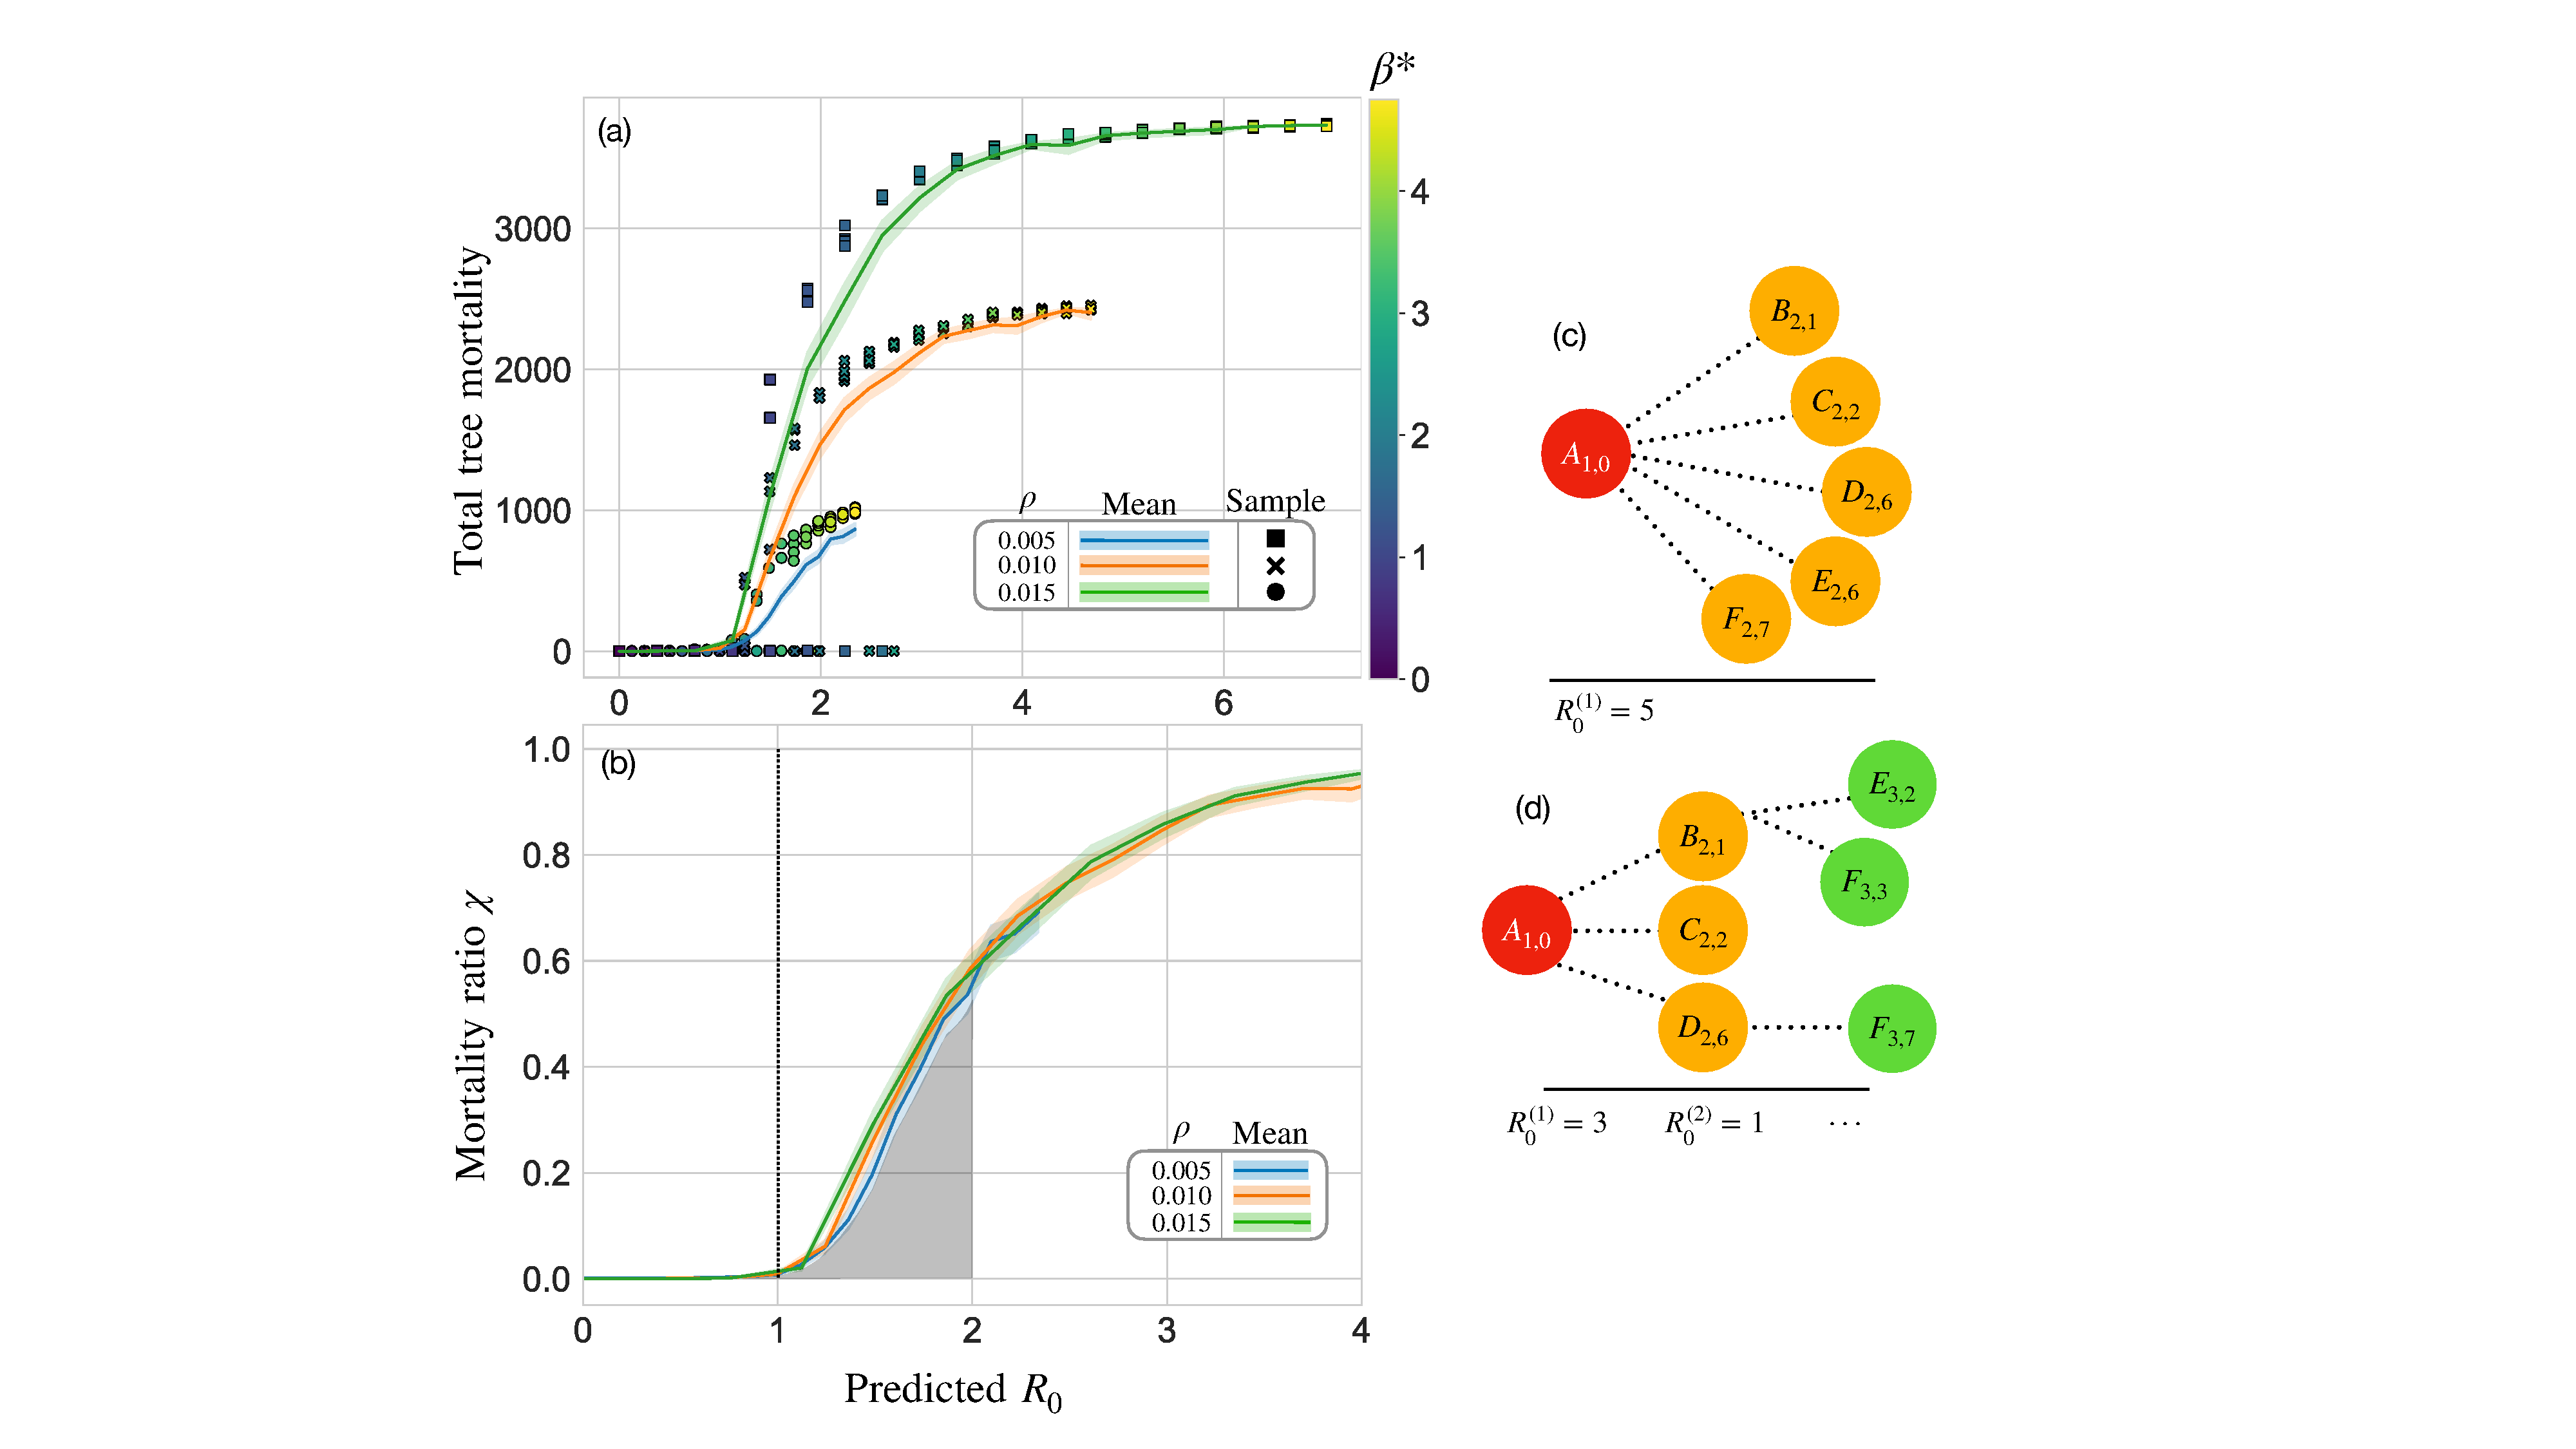
\includegraphics[scale=0.44]{chapter5/figures/fig4-R0-analytic-vs-mortality.pdf}
    \caption{The relationship between the total tree mortality and the predicted $R_0$ value. (a) For three values of tree density and multiple infectivity values, the ensemble-averaged tree mortality (as a continuous solid line) is overlaid with a small sample of data points shown by the scatter plot. The shape and colour of each data point indicate the tree density and infectivity, respectively. (b) The fraction of removed trees as a fraction of the population is plotted against mortality the analytical value of $R_0$. Together panels (a) and (b) demonstrate a threshold-like behaviour at $R_0=1$. (c) A graphical representation of the idealised $R_0$ approximation, as per equation \ref{eq:Appendix_final_expression1}. (d) A more realistic network representing the epidemic branching process. In both panels, the arrow of time is left to right, and subscripts reflect the generation and time-step that trees become infected.}
    \label{fig:R0-vs-NLM-sims}
\end{figure}

Figure \ref{fig:R0-vs-NLM-sims}(a) shows the relationship between tree mortality, the predicted $R_0$ from equation \ref{eq:Appendix_final_expression1}, and the two epidemic parameters $\rho$ and $\beta$.
A scatter plot of coloured data points (depicting a small sample of data) overlays a continuous line representing an ensemble average. 
The corresponding colour bars on the scatter plot and ensemble-average characterise infectivity and density, respectively.
The Figure illustrates that tree mortality remains low when $R_0 < 1$ and $\beta$ is small, as indicated by coloured scatter plots in blue. Conversely, the tree mortality increases with infectivity when $R_0>1$, shown by the yellow scatter points. Therefore, equation \ref{eq:Appendix_final_expression1} demonstrates a threshold-like behaviour defined by $R_0=1$.
Above the threshold $R_0=1$, increasing the tree density increases the epidemic scale because more susceptible hosts are available to infect, as indicated by the significant rise in tree mortality in the continuous green line. 

Despite being above the threshold, the numerical simulations can still fail to produce an epidemic,
illustrated by the small number of data points beyond $R_0=1$ that map to a zero-sized epidemic. For example, at $R_0\approx 2$ a small number of points can far below each ensemble mean.
Similarly, the ensemble mean is lowered by pathogen extinction\textemdash demonstrated by slight differences between the collection of points and the ensemble mean in the interval $R_0 \in [1, 3]$.
These observations result from the fact that under the influence of early stochastic forces, the probability of epidemic extinction is higher \cite{perspectives-on-r0, R0-perc-ref}, which unfortunately marks a flaw in the concept of $R_0$ in general \cite{li2011failure}.

Figure \ref{fig:R0-vs-NLM-sims}(b) presents the same essential information as Figure \ref{fig:R0-vs-NLM-sims}(a).
Although, the ensemble mean is plotted against the mortality ratio (i.e. the total number of removed trees as a fraction of the total population), denoted by $\chi$.
Given that each ensemble mean converges to the same epidemic scale, the quantity $\chi$ demonstrates utility when accessing the epidemic impact between different tree-densities.
Consequently, the threshold $R_0=1$ is easily observable in Figure \ref{fig:R0-vs-NLM-sims}(b), indicated in shaded grey.
The threshold-like behaviour witnessed in Figures \ref{fig:R0-vs-NLM-sims}(a-b) demonstrate that equation \ref{eq:Appendix_final_expression1} provides a simple predictive framework for the  NLM.
That said, more complicated dynamics\textemdash such as exponential lifetimes, elaborate dispersal kernels or host aggregation\textemdash could significantly hinder the analytic solution proposed in section \ref{sec:r0-derivation}.

Another limitation to the equation \ref{eq:Appendix_final_expression1} can be explained by Figure \ref{fig:R0-vs-NLM-sims}(c), which shows a typical NLM simulation used to access the analytic expression of $R_0$.
Namely, a single `fist-generation' infected tree at time $t=0$ ($A_{1, 0}$) that happens to infect a number of neighbouring trees ($B_{1,1}$ to $G_{1, 7}$).
According to the $R_0$ approximation, the local density reductions due to $B_{2,1}-G_{2, 7}$ are neglected, and $A_{1, 0}$ remains the only active source of infection.
Neglecting the influence of other secondary infected hosts helped to keep analytical derivation simple.
But for highly infectious outbreaks, equation \ref{eq:Appendix_final_expression1} is likely to overestimate $R_0$.
Figure \ref{fig:R0-vs-NLM-sims}(d) can be used to understand why overestimates of $R_0$ are likely.
In Figure \ref{fig:R0-vs-NLM-sims}(d), non-trivial density reductions could be expected from the second and third generation of infected hosts, $B_{2,1}, C_{2, 2}, D_{2, 6}$ and $E_{3, 2}, D_{3, 5}, D_{3, 6}$ respectively\textemdash here, the first subscript refers to time and the second subscript refers to the generation\textemdash 
leading to an environment where the primary infected host $A_{1, 0}$ has less neighbours to infect.
Given these limitations, a and more flexible method of calculating $R_0$ is investigated in the next section.

\section{Contact-tracing secondary infections}
\label{sec:contract-traced-R0}

% reference for network model of secondary infections \cite{PAUTASSO2010424} r
In this section an alternate method of calculating $R_0$ is presented that incorporates the effect of secondary infections  
(up the $n^{th}$ generations), analogous to contact-tracing emerging epidemics in human populations \cite{eames2003contact}.
By collecting individual tree-to-tree induced secondary infections, the entire history is captured, illustrated graphically in Figure \ref{fig:R0-vs-NLM-sims}(d).
At $t=0$, the first generation primary infected tree, denoted by $A$, produces three $2^{nd}$ generation infections $B$-$D$ in orange that in turn produce
third generation infections are shown in green.
The contact-traced $R_0$ can be defined by:

\begin{defn} % look into definitions of next-generation operator
\label{def:R0_contact_traced}
\textit{at $t=0$, simulations begin with one or more infected hosts, and the entire epidemic history captures which host infects which others.
The mean number of infections that result for each generation $i$ is computed and denoted by $R^{(i)}_0$.}
\end{defn}

In Figure \ref{fig:contact-trace}(a), observations from the (ensemble-averaged) contact-traced $R_0$ is shown for $10$ generations and 
four infectivity parameters; in all plots, tree densities, dispersal kernel and domain sizes remain fixed ($\rho=0.01, \ell=50, \mathcal{L}=500$).
For highly infectious outbreaks, the host population quickly decreases, and $R^{(i)}_0$ begins high and gradually decreases with each generation.
In contrast, for infectivities just above the threshold $R^{(i)}_0$ remains approximately stable with each generation because the population of susceptible hosts remains high.  
For all boxes in Figure \ref{fig:contact-trace}(a), the interquartile range decreases with the generation, suggesting that early stochastic forces increase the spread of $R^{(i)}_0$ values.
The number of secondary-infected trees will therefore vary over time and mirror the host population.
Had the re-growth of susceptible trees been considered, $R^{(i)}_0$ can be speculated to behave very differently for later generations.

% 1) Here $R_0$ is just above threshold for earlier times and barely spreads, however, the spread is chaotic. %
% 2) From Figures \ref{fig:contact-trace}(b-d), we have demonstrated that this definition of $R_0$ %
% reliably captures the threshold of transmission during the initial stage of infection. %
% Undesirably, we have made simplification in the assumptions and have not achieved a complete %
% characterisation of $R_0$\textemdash which could, in be defined in terms of a growth %
% rate per generation \cite{R0-construct}. %

Figure \ref{fig:contact-trace}(b) compares the ensemble-averaged $R^{(i)}_0$ values, shown in Figure \ref{fig:contact-trace}(a),
to predictions from the analytic expression for $R_0$.
Analytic $R_0$ values are plotted as horizontal dashed lines, and each $R_0^{(i)}$ ensemble average (shown by the solid lines) is surrounded by shaded bounds reflecting a $95\%$ confidence interval.
For the lowest infectiviy parameter around the threshold $R^{(i)}_0=1$, shown in blue, the contact-traced value of $R_0$ compares well with equation \ref{eq:Appendix_final_expression1}.
However, increasing the infectivity to $\beta^*=2$ (in orange) equation \ref{eq:Appendix_final_expression1} agrees well for early generations, but deviates for later generations, 
revealed by comparing the dashed horizontal and solid orange lines.
Deviations only grow larger as $\beta^*$ increases.
That is to say, looking at the green and red lines in Figure \ref{fig:contact-trace}(b), one can confirm that equation \ref{eq:Appendix_final_expression1} does indeed overestimate pathogen transmissibility.
Although significant disparities exist, Figure \ref{fig:contact-trace}(b) implies that both analytic and contact-traced reproductive ratios agree on the threshold $R_0=1$.

\begin{figure}
    \centering
    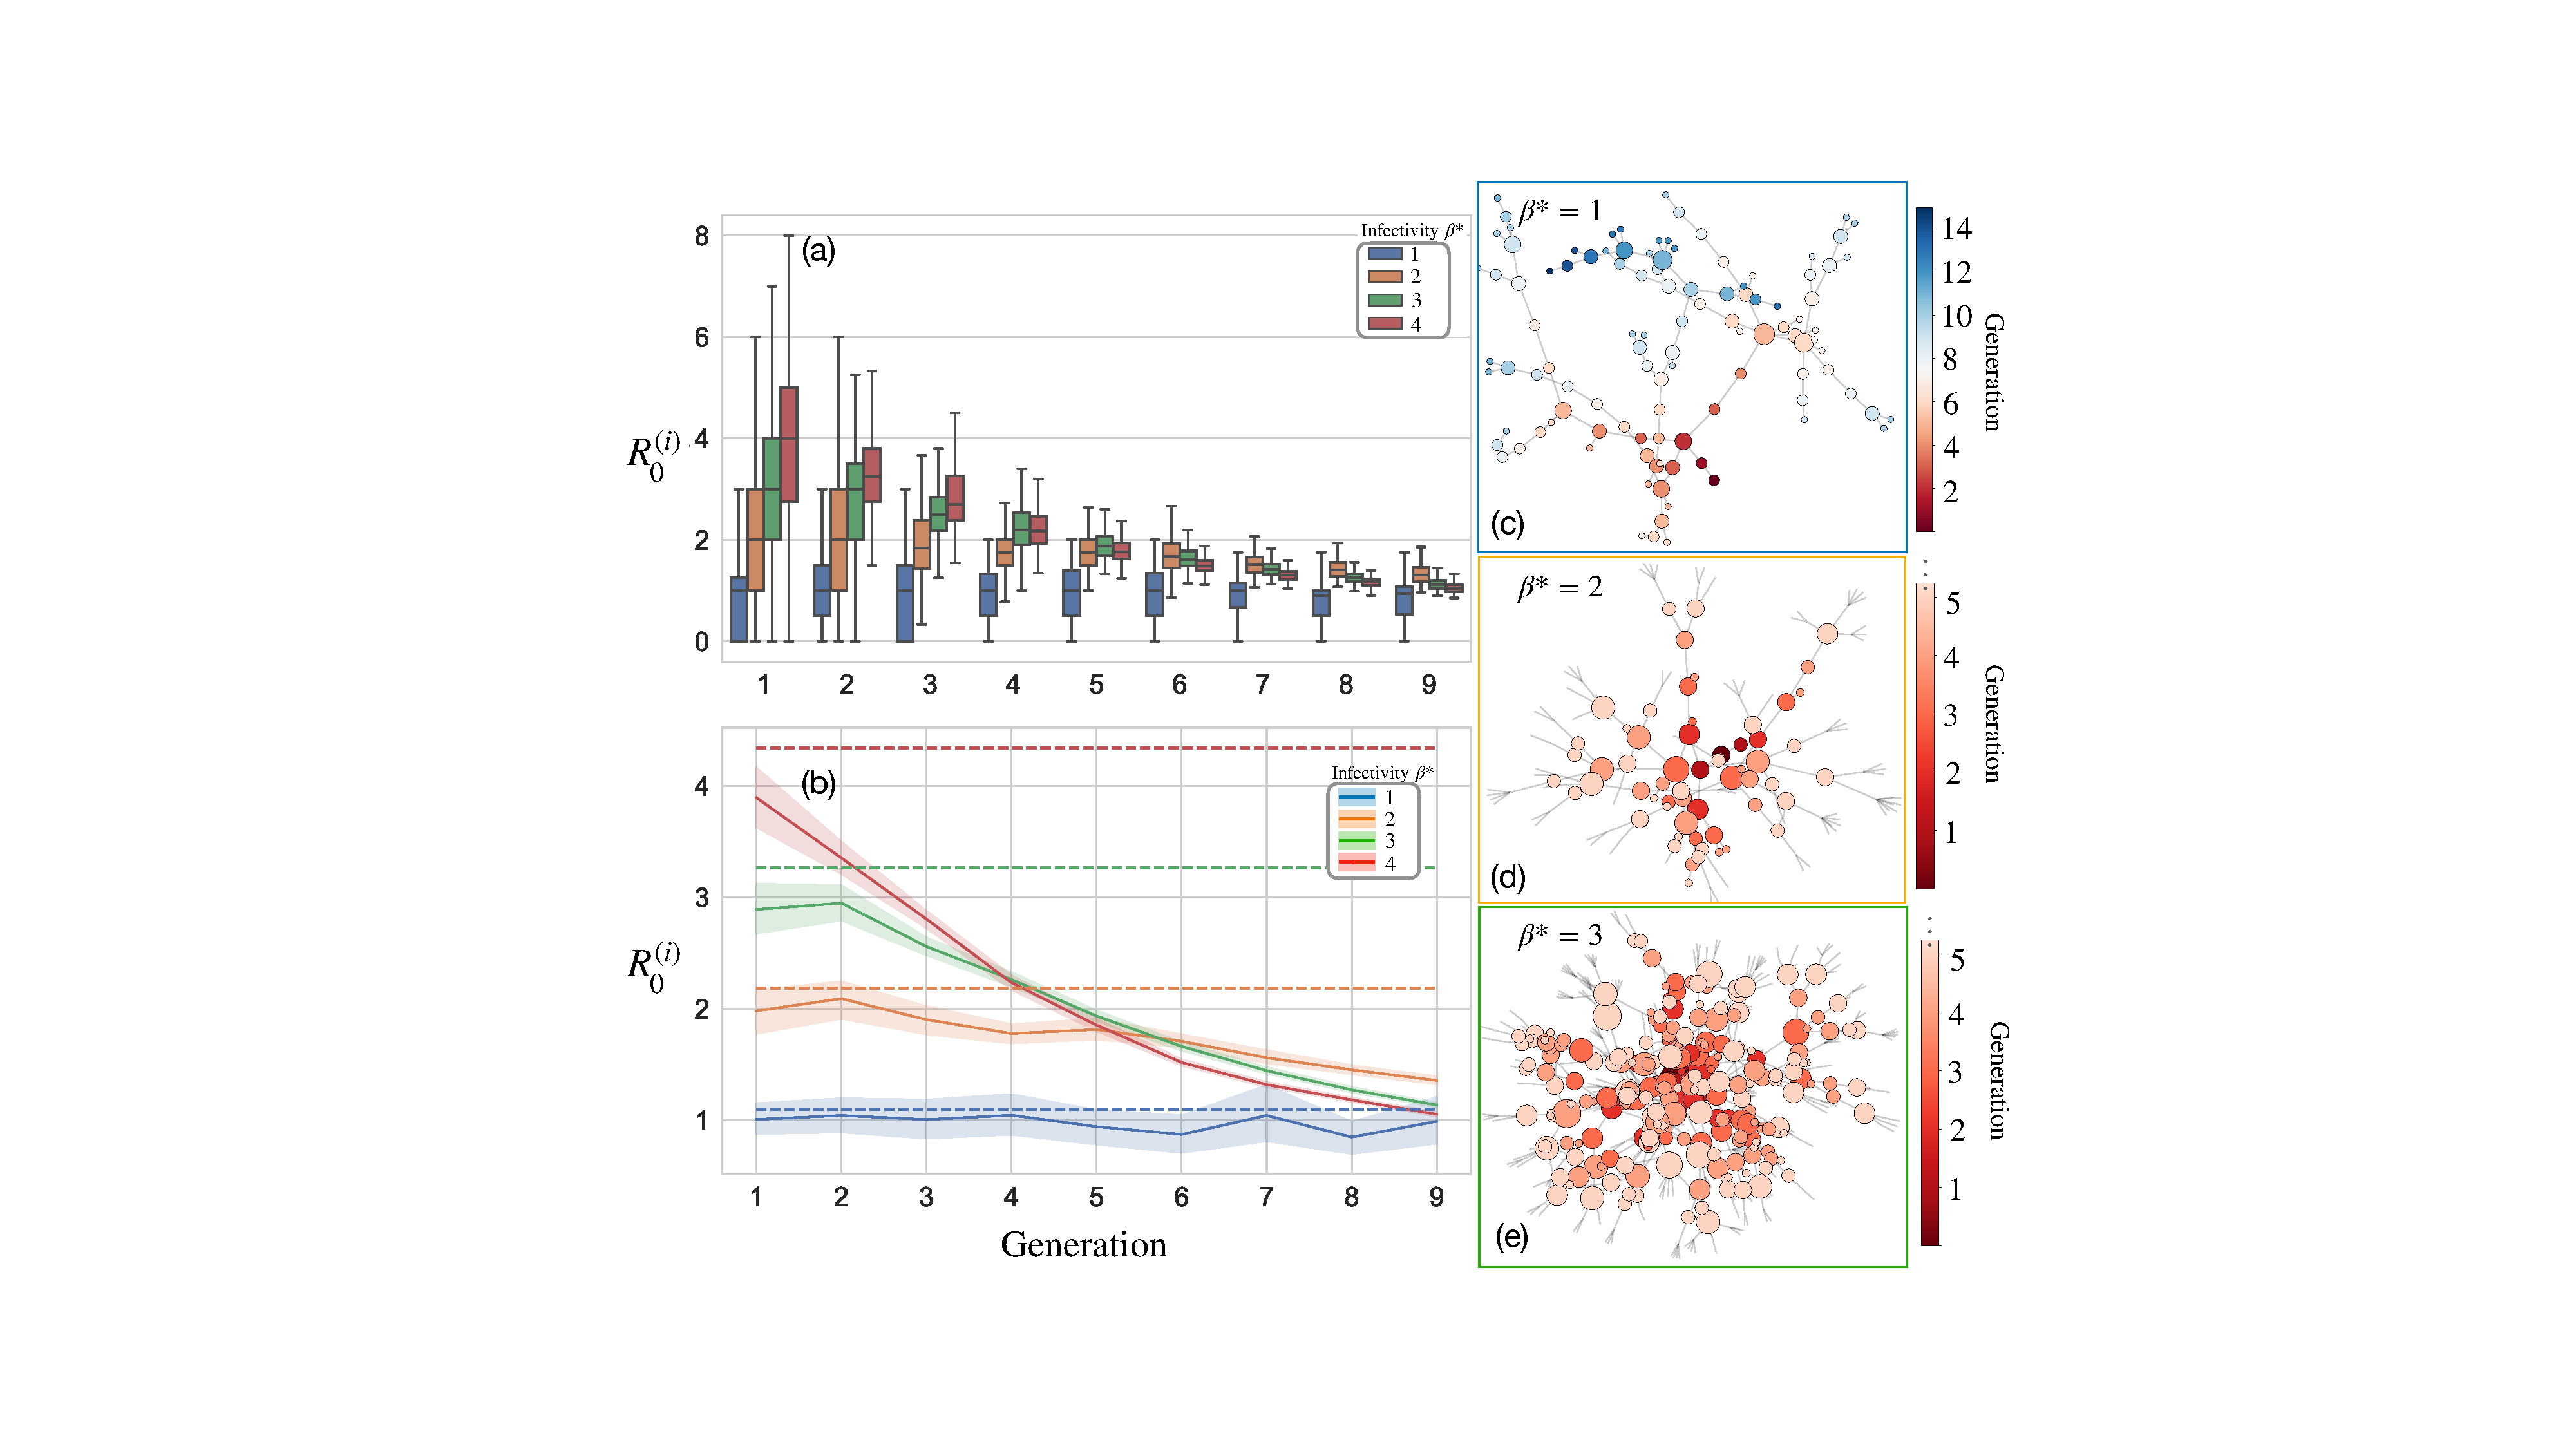
\includegraphics[scale=0.475]{chapter5/figures/fig5-R0-contact.pdf}
    \caption{Contact-tracing mean number of secondary infections for the $i^{th}$ generation of infected trees, $R^{(i)}_0$. For all simulations, tree densities are fixed along with dispersal kernels, ($\rho=0.01$) and $\ell=50$ respectively, inside a domain of size $\mathcal{L \times L} = 500 \times 500$.
    (a) A box and whisker plot showing the mean number of secondary infections plotted over $10$ generations over an ensemble of size $N=500$. Four different infectivity values are shown, from blue to red. (b) The ensemble-mean in (a) is compared against predictions from the analytic expression of $R_0$, plotted as horizontal dashed lines. For early generations, equation \ref{eq:Appendix_final_expression1} agrees well with the contact-traced value of $R_0$ but overestimates the spread for higher infectivities. (c-e) A network diagram representation of typical simulations for parameters $\beta^* \in \lbrace 1, 2, 3 \rbrace $. The nodes' colour and size reflect the generation and number of secondary infections, respectively. As $\beta^*$ is increased, the network quickly explodes\textemdash, thus reflecting the complexity of controlling highly infectious outbreaks.}
    \label{fig:contact-trace}
\end{figure}

Simplistic interactions between trees permit an alternative network representation of disease spread.
In Figures \ref{fig:contact-trace}(c-e), a directed network of disease spread is shown for three typical simulations with infectivity parameters $\beta^* \in \lbrace 1, 2, 3 \rbrace$.
Nodes depict individual trees, while colour and size represent the generation infected and the number of induced secondary infections.
Between two nodes, one edge connects infected generations $n$  and generation $n+1$ (arrows showing the direction are omitted for visual clarity). 
When epidemic parameters are around the threshold, as in Figure \ref{fig:contact-trace}(c), the network appears sparse and chaotic;
whereas Figures \ref{fig:contact-trace}(d-e) show that if infectivity is increased, the network proliferates rapidly. 
Indeed for $\beta^*=2$ and $\beta^*=2$ the network became large if plotted for all generations\textemdash consequently $R_0^{(5)}$ was truncated to permit visualisation.

From Figures \ref{fig:contact-trace}(d-e), one can discern assumptions implicit within the NLM and visualise how targeted epidemic control might be optimised. In the NLM, tree-to-tree interactions are particle-like, meaning that infections spread unidirectionally between two trees at any time. In real life, interactions are more complex. For example, consider two infected trees $(A, B)$ in the vicinity of one healthy susceptible neighbour $C$. Here, infection pressure on $C$ is likely a continuous function of $A$ and $B$. We can collectively represent these more complex interactions by multiple edges between $A, B$ and $C$ in a network diagram.
However, the probability of $C$ becoming infected by $A$, $B$ (or $A \cap B$) occurs with statistical independence. Therefore, we employ the standard method of combining statistically independent events from the inclusion-exclusion formula\textemdash given in appendix \ref{A:combiniing-probabilities}. 

Despite the necessity of modelling the simultaneous infection pressure from multiple infected trees, it complicates the definition of $R_0$.
Primarily, infections can originate from multiple sources, and we cannot tell from which tree(s) the infection initially spread. See appendix \ref{A:combiniing-probabilities} for a more in-depth discussion on combining probabilities. Nonetheless, another assumption relates to self-loops in the network. In the framework proposed here, trees transition into the $R$ compartment and self-loops are negated. However, in reality, re-infection is possible (e.g. the yearly cycle of ash dieback \cite{gross2014h}) that could be supposed to cause a host's infectivity to increase with each re-infection.

The networks shown in Figures \ref{fig:contact-trace}(d-e) present a simple, yet insightful, representation to gauge what connections epidemic control would need to disrupt.
Well-known results suggest that the scale of control should reflect the spatio-temporal scale of disease spread \cite{control-scale-matching}.
In Figure \ref{fig:contact-trace}(d), even a minimal control effort might disrupt the network well below the threshold of spread,
whereas Figures (d) and (e) would incur an increased effort to stop the spread.
In the network representation, optimised control would involve targeting high priority links between nodes;
this reflects various methods that aim to optimise control by identifying high-risk hosts.


\subsection{Contact-traced $R_0$ and tree mortality}

In Figure \ref{fig:contact-trace-vs-mortality}, the contact-traced value of $R_0$ is compared against the tree mortality, similar to the previous analysis in section \ref{sec:tree-mortality-analytic}.
Figure \ref{fig:contact-trace-vs-mortality} shows an ensemble-averaged reproductive ratio (up to $R_0^{(i=5)}$) plotted against the mean tree mortality, indicated by the dashed curves.
The ensemble mean is then overlaid with a coloured scatter plot depicting a small sample of the data.
Each simulation in Figure \ref{fig:contact-trace-vs-mortality} was repeated $10^3$ times for fixed density $\rho=0.01$, dispersal $\ell=50$ and $\mathcal{L}=500$ over $2500$ time-steps.
As before, a threshold can be witnessed at $R_0^{(i)}=1$, above which tree mortality rises steeply.
For $R_0^{(1)}$, the threshold phenomena witnessed in Figure \ref{fig:contact-trace-vs-mortality} (shown in dashed blue) appears similar to the previous analytic $R_0$ examination.
However, each successive generation appears to define a sharper threshold, especially when $\beta^*$ is high, suggested by the steeper coloured dashed curves.

The steeper thresholds witnessed in Figure \ref{fig:contact-trace-vs-mortality} can be understood
by considering initial stochasticity.
If an outbreak (with high $\beta^*$) does not become extinct at early times, the epidemic is likely to continue to spread until no susceptible trees are left to infect.
Hence, epidemic impact is high and the threshold is sharp for $R_0^{(i)}$, where $i > 1$. 
The reader is referred back to the network diagrams shown in Figure \ref{fig:contact-trace}(d-e) to gain intuition behind this idea;
if the pathogen survives beyond the initial outbreak to establish new centres of infection, the network quickly explodes, and pathogen extinction is unlikely.

The ensemble shown in Figure \ref{fig:contact-trace-vs-mortality} was re-run with $10$ centrally-located initial infections at $t=0$ to test the initial stochasticity.
Intuitively, increasing the number of infected trees reduced early extinction events and subsequently raised the mean tree mortality.
In addition, raising the number of initially infected trees reduced stochasticity in the ensemble and presented a more abrupt threshold in comparison to Figure \ref{fig:contact-trace-vs-mortality}\textemdash more information can be found in Appendix \ref{A:R0-contact-traced-mortality}.

\begin{figure}
    \centering
    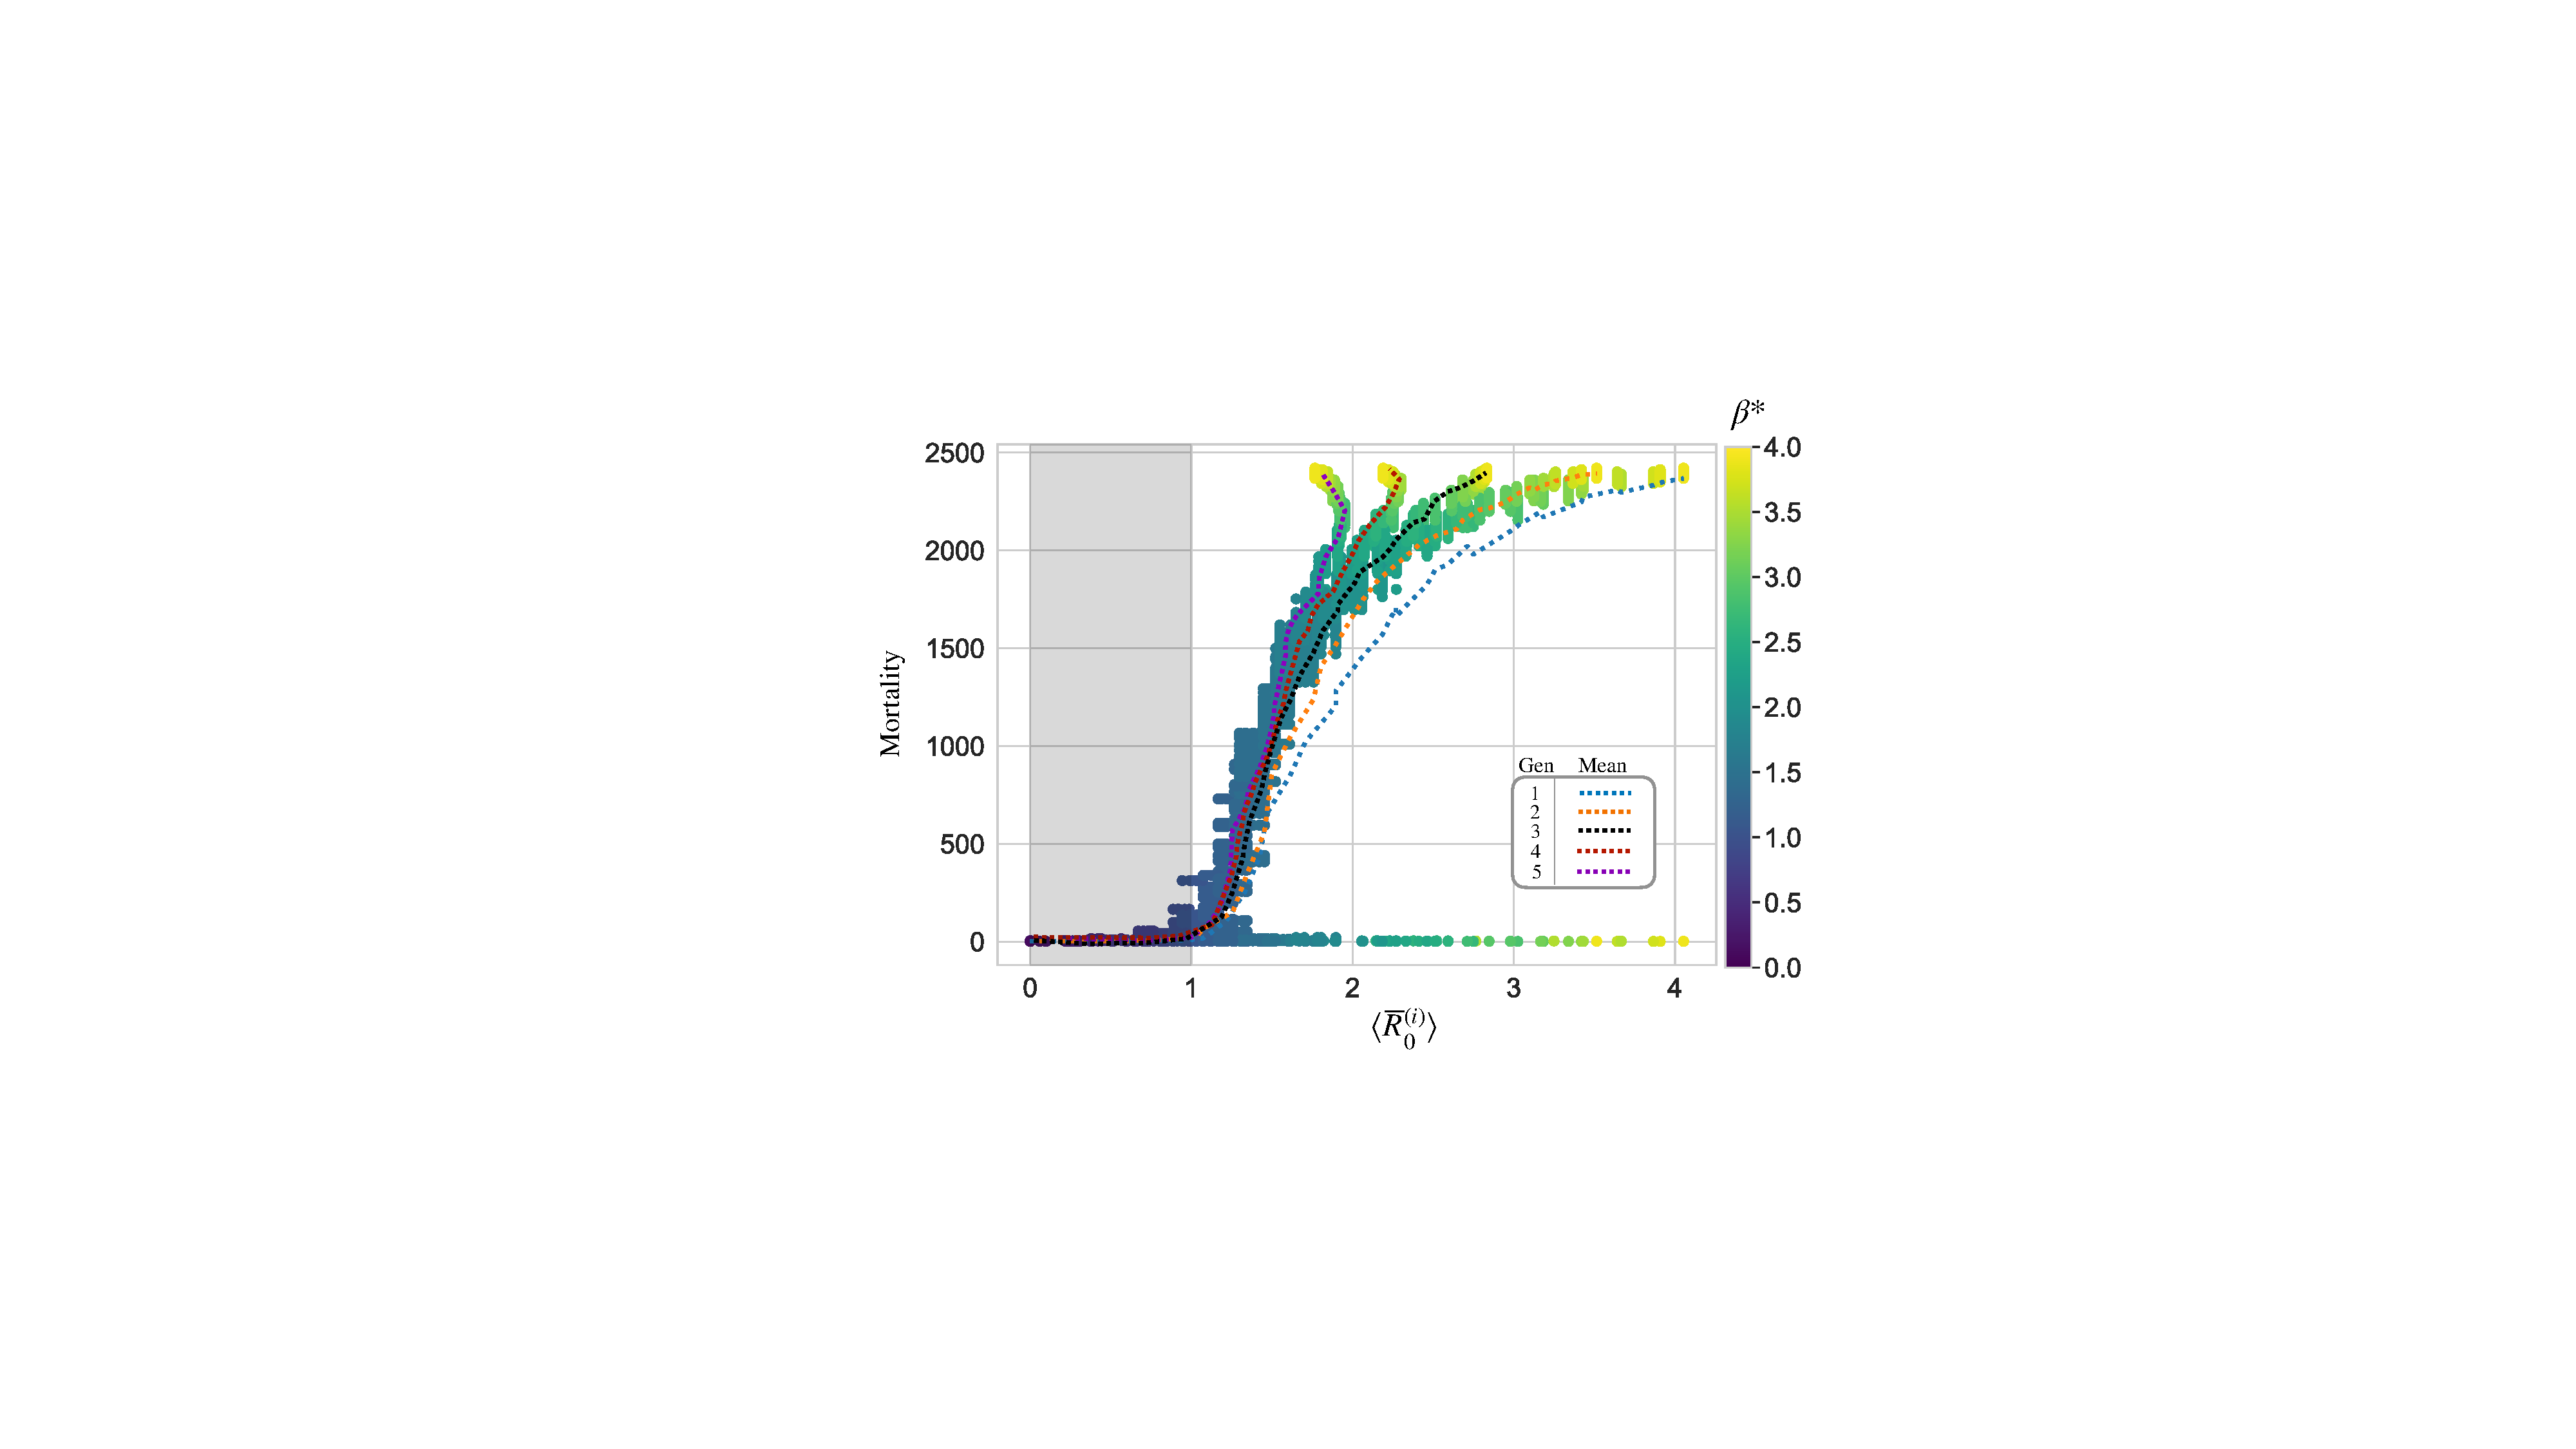
\includegraphics[scale=0.6]{chapter5/figures/fig6-R0-contact-vs-mortality.pdf}
    \caption{Comparing the contact-traced reproduction ratio and the total tree mortality. 
    In each simulation, the tree density and dispersal kernel was fixed to $\rho=0.01$ and $\ell=50$, respectively. 
    For each value of infectivity $\beta^*$, the ensemble-averaged value of $R_0^{(i)}$ is plotted against the mean tree mortality, shown by the dashed curves, for five generations, i.e. $R_{0}^{(5)}$.
    A coloured scatter plot overlays the ensemble-averaged line plots showing a sample of the data\textemdash and also reflecting the value of $\beta^*$.
    As before, a threshold arises around $R_0^{(i)} = 1$, although this time the threshold appears steeper.}
    \label{fig:contact-trace-vs-mortality}
\end{figure}

\newpage
\section{Discussion and future work}

The main aim of this Chapter was to construct a more realistic, dispersal-based model of tree disease.
Hence, a non-local dispersal model (NLM) of tree disease was constructed with SIR compartments and a Gaussian kernel.
Notwithstanding its generic construction, the NLM provides a foundation for the remaining chapters in this thesis.
After describing the NLM, it was compared to the standard SIR framework for a number of dispersal length scales and domain sizes.
Despite some differences, the NLM compared more favourable with the SIR model when the dispersal scale parameter was comparable to the domain size.
Comparisons, therefore, provide compelling indications that spatially-explicit contact-mixing in the tree population may arise with sufficient dispersal.
From this observation, we may question the utility of spatial models for systems where the dispersal length scale is comparable to the size of domain, e.g. when modelling the spread of disease in small fields or plantations. However, comparisons to the SIR model were simplified and limited to one parameter (i.e. the ratio $\beta/\gamma$). As such, the analysis constitutes a preliminary result, and a more sophisticated comparison method is required to glean further insight. For example, a better method of might involve using inference (MCMC methods) to fit the NLM against the standard SIR model.

Two methods of calculating a reproduction ratio, one analytic ($R_0$) and one numerically contact-traced ($R_0^{(i)}$), were outlined to categorize the NLM.
The analytic threshold predicted by equation \ref{eq:Appendix_final_expression1} agreed well with the `actual' contact-traced reproduction ratio computed through NLM simulations,
caveat-ed by the observation that it tends to overestimate $R_0$ when epidemic severity is high.
The overestimation of $R_0$ can be compared to well-known results by \cite{R0-perc-ref, doi:10.1098/rsif.2005.0051},
who showed that the first-generation basic reproduction ratio for farms infected with foot-and-mouth overestimates the growth rate of infection.
In addition, \cite{R0-perc-ref} found that the second generation of infected farms gave a better predictor of the final-sized epidemic (conditional on the epidemic occurring),
thus presenting a clear link to our observation that the tree mortality threshold defined by $R_0^{(i)}=1$ was sharper for later generations.
Crucially, each method of calculating the reproduction ratio defined a threshold around unity, beyond which epidemic impact becomes non-trivial.

An attractive feature of the contact-tracing method, as per definition \ref{def:R0_contact_traced}, 
pertains to its flexibility in the face of more complex spatially explicit models.
Analytical solutions of $R_0$ may become hard to determine for more elaborate life-cycles, dynamics and aggregated host distributions.
Although contact-tracing provides an easy-to-implement method of calculating $R_0^{(i)}$, it should remain, first and foremost, an abstract modelling tool.
For example, consider the immense difficulty of experimentally contact-tracing secondary infections when an epidemic spreads through a forest/landscape.
Contact-tracing the reproduction ratio can therefore be presumed as unobservable in nature\footnote{
We may speculate about measuring a time-varying reproduction number based on the observed numbers of infected hosts,
a well-known concept for characterizing epidemic transmission in human populations \cite{thompson2019improved}.}
However, given sufficient data, one might fit a value of $\beta$ and reverse-engineer a value of $R_0^{(i)}$ from the model;
which leads us to a discussion around the infectivity parameter $\beta$.

A probability of state-change represents infectivity in the NLM, which followed naturally from the percolation model outlined in section \ref{ch3:two-param-model} \cite{OROZCOFUENTES201912}.
However, growth rates are usually employed to describe infectivity\textemdash going back to the original SIR framework \cite{kermack-model} and the logistic growth model of \cite{van2013plant}.
The approach adopted in this Chapter is, therefore, a-typical of contemporary dispersal models based on rates, e.g. \cite{fabre2021optimising, control-theory, white2017modelling, large-scale-control}.
Given that growth rates parameterize most diseases in the literature, the NLM might arguably require a modification towards a rate-based implementation;
however, it must be remarked that sometimes this may not be needed, given that measuring growth rates\textemdash particularly for time-varying infectivities\textemdash is extremely difficult \cite{13-challenges}.
Although unconfirmed, we may suppose an equivalence between the infectivity $\beta$ and an emergent growth rate. This assertion is supported by the similarities exhibited between the NLM and the rate-based standard SIR model in Figure \ref{fig:SIR-fitting} (in addition to appendix \ref{a:exponentially-distributed-lt}).
Nevertheless, presenting $\beta$ as a probability describes an intuitive low-level (microscopic) perspective of disease spread which would, 
in theory, be observable/measurable in reality, in contrast to the $R_0^{(i)}$.
Hence, we may consider infectivity $\beta$ as a fitting parameter.


\newpage
